
\chapter{多個語音離散表徵與音位的關係}   \newcommand{\jefftablesep}{\vspace{0.5cm}}
\renewcommand{\arraystretch}{0.7}
\newcommand{\jcm}[1]{}


% \newcommand{\jefftablesep}{\vspace{0.5cm}}\renewcommand{\arraystretch}{0.7} % 調整行高

\section{動機}

  如第三章所述,一個文字或音位往往對應到上百毫秒的語音訊號,然而單一離散單元所對應的聲音訊號為 10 或 20 毫秒,亦即同一段語音所對應的離散單元數目將比音位或文字多出許多。本章節從自然語言處理中獲取靈感,將文字處理中的分詞演算法(Tokenization)應用於離散單元序列上,使得離散單元重新組合成次詞單位(Subword Units),稱之為「聲學片段(Acoustic Piece)」,以這些由多個離散單元組成的符記(Token)\footnote{指資料序列中的離散基本單位。}作為新的基本單位重新編碼語音訊號,取代原先的離散單元。為了分析聲學片段是否更接近音位的序列,在此將續用上一章節的分析方法,比對並檢驗引入次詞單位是否有機會得到更好的語音表徵,進而有機會用於無文字(Textless)架構\cite{lakhotia_generative_2021, lakhotia_generative_2021-1, noauthor_textless_2021}中。

\section{相關研究} 

  在無文字架構被提出後的約兩年後,藉助次詞單位組合離散單元的研究逐步出現。任氏(Ren)等人 \cite{ren_speech_2022}\citetag{1-22A4-Pretrain-ap})最先提出聲學片段的概念,該論文比對離散單元序列及對應的文字轉寫,從中觀察到許多相似的規律重複出現,而且不限於單一語者。受此啟發,本論文首先將離散單元,透過文字處理中常用以獲得次詞單位的「句片段(SentencePiece) \cite{kudo_sentencepiece_2018} 套件獲得新的符記 --- 「聲學片段」,並用於語音辨識的預訓練上。

        不久,由吳氏(Wu)提出的 Wav2seq \cite{wu_wav2seq_2023}\citetag{2-22A5-wav2seq}論文中,考量文字與語音的序列長度差異,並基於離散單元和音位的關聯性,將離散單元視為字符(Character),嘗試將這些字符透過次詞單位組成「虛擬語言(Pseudo-language\footnote{偽語言對應之離散單元被視為「虛擬文字(Pseudo-text)」})」,來幫助語音到文字的模型。在實際應用中,因為解碼器生成的目標文字序列亦是由次詞單位組成,因此該篇研究旨在讓模型在預訓練後可以快速適應下游任務。與前一篇呼應,聲學片段對語音預訓練的效果在\cite{10096788}\citetag{3-23A-coarser-grain}中被探討,此後聲學片段更被應用於縮短資料序列長度\cite{chang_exploration_2023}\citetag{4-23B-Exploration of Efficient End-to-End ASR using Discretized Input from Self-Supervised Learning} 、語音生成\cite{shen2024acoustic}\citetag{5-24A-speech-gen},或學習更穩健(Robust)的語音表徵\cite{chang2023r}\citetag{6-23B-rspin-acousticpiece}。

        近期,張氏(Chang)等人\cite{chang_exploring_2024}\citetag{7-23B-shinji-hsiuhsuan}將以分詞方法處理離散單元的流程(Pipeline)納入 ESPNet 套件 \cite{watanabe2018espnet} 中,並在語音辨識、語音翻譯等任務中獲得了超越以往的表現,進一步證明了這個方法的效果。

\section{文字處理中的分詞演算法}

  在以文字為主體的自然語言處理中,文字文本除了以單詞(Word)或字元(Character)為處理單位,更常見的作法是透過分詞演算法(Tokenization)將文本分段,以「次詞單位」構成詞彙表來重新編碼文本,用於文字模型的訓練與推理。

        使用次詞單位的優點包含:

\begin{enumerate}
    \item 固定詞彙表大小,避免未登錄詞(Out-of-vocabulary,OOV)
    \item 縮短資料序列的長度,提升訓練和推論的效率。
    \item 分解單詞,捕捉更細緻的語意關係,模擬如英語中的字首(Prefix)、字尾(Suffix)等等具有特定意義的文字組合。
\end{enumerate}

\subsection{常見演算法}

  以下介紹幾種常見的分詞方法:

\paragraph{位元組對編碼(Byte Pair Encoding,BPE)} \hfill \break
%
  位元組對編碼 \cite{10.5555/177910.177914, sennrich_neural_2016} 是一種常用的分詞方法,最初來自資料壓縮技術 \cite{10.5555/177910.177914},後來被引入到自然語言處理領域,用以處理機器翻譯問題 \cite{sennrich_neural_2016} 。
該演算法從字元開始,根據詞彙表中各個次詞單位的頻率,反覆合併常見的字元成為新的次詞單位,直到達到預定的詞彙表大小。

\paragraph{單詞片段(WordPiece)} \hfill \break
%
  WordPiece \cite{wu2016google} 演算法由 Google 用以訓練機器翻譯系統,並在 BERT \cite{devlin_bert_2019} 模型中被使用而廣為人知。與位元組對編碼相似,同樣是透過反覆合併的策略,但合併的依據改以機率模型取代出現頻率。

\paragraph{單一詞語言模型(Unigram Language Model)} \hfill \break
%
  單一詞語言模型 \cite{kudo2018subword} 是基於語言模型的分詞方法,以機率分佈選擇次詞單位,並以最大化輸入文本的機率來為文本分段。

\subsection{「句片段(SentencePiece)」套件}

  「句片段(SentencePiece) \cite{kudo_sentencepiece_2018}
」是由 Google 開發的分詞套件,實作了前述的位元組對編碼和單一詞演算法。其優勢在於可應用於不同語言,尤其用於處理中文、日文等不使用空格分隔單詞的語言文本時,此套件大大的簡化了前處理的流程。
        考慮到語音訊號本身不如英語等文字,在書寫時就已經具備空格分隔單詞,因此本章節的所有次詞單位皆以句片段套件中的單一詞演算法取得。

\section{分析方式}

  本章節沿用上一章節 LibriSpeech 資料集的 train-clean-100 訓練子集,以單一詞演算法取得次詞單位,並嘗試 500、1000、8000、10000、20000 五種符記種數,對每一種語音表徵和 K-平均模型的分群數,各自取得五種聲學片段文本。

        比照第三章的分析方式,本章除了整體的純度與相互資訊數據外,亦同樣從聲學片段與音位的角度分別探討,藉由調整次詞單位的種類數量,探討引入次詞單位並改變符記數量,將如何影響這些符記序列與音位標註間的相關性。然而,為了避免結果呈現過於複雜,細部分析時將著重比對 500 和 1000 種次詞單位的結果變化。

        由於本章節探討重點為次詞單位種數變化的影響,延續第三章的發現,後續分析將以表現最好的 HuBERT 離散表徵為主。在需要比較離散單元分群數影響時,我們將比對分群數為 50 與 100 時的差異,否則為避免數據過於複雜,離散單元的分群數預設為 50 進行細部探討。

\section{分析結果} 

  承繼上一個章節的分析方法,我們先將純度等數據與條件機率熱圖 $p_{y|z}(i | j)$ \footnote{由於共同機率分佈熱圖 $p_{yz}$ 的數值對於觀察符記對應到音位的關係較不明顯,因此仿照 SpeechTokenizer \cite{zhang2024speechtokenizer}、DinoSR \cite{liu2024dinosr} 等論文使用 $p_{y|z}(i | j)$ 呈現。} 兩者互相對照,並以語音學排序呈現,觀察聲學片段與音位之間兩者的分佈關係。

\subsection{由聲學片段角度探討}
{
\subsubsection{聲學片段數量的影響}

{
    {
        \newcommand{\tempwidth}[0]{0.8\linewidth}
        \begin{figure}
             \centering
             \begin{subfigure}{\textwidth}
                 \centering
                 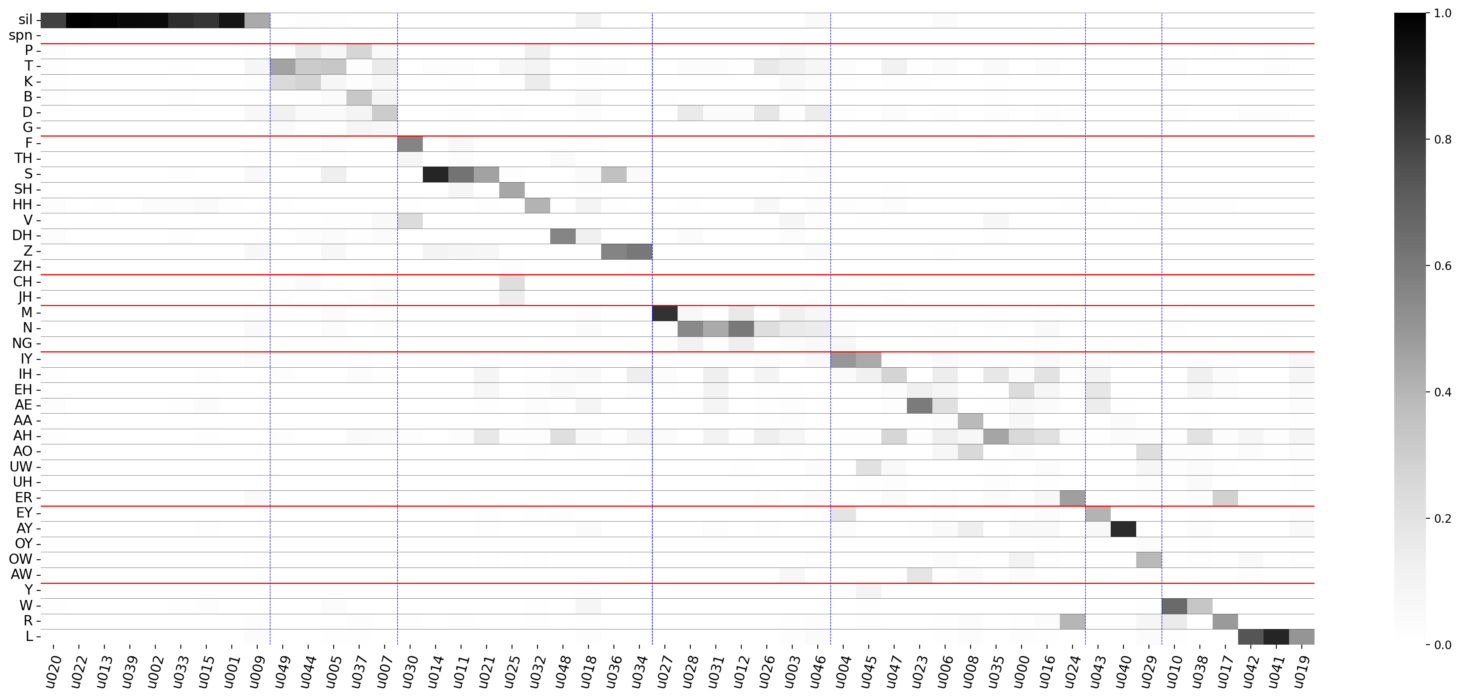
\includegraphics[width=\tempwidth]{feasiblefigs/ch4figs/hub-u050-ap0000-givenunit-byphn.png}
                 \caption{離散單元}
                 \label{fig:hub-u050-ap0000-givenunit-byphn}
             \end{subfigure}
             \vfill
             \begin{subfigure}{\textwidth}
                 \centering
                 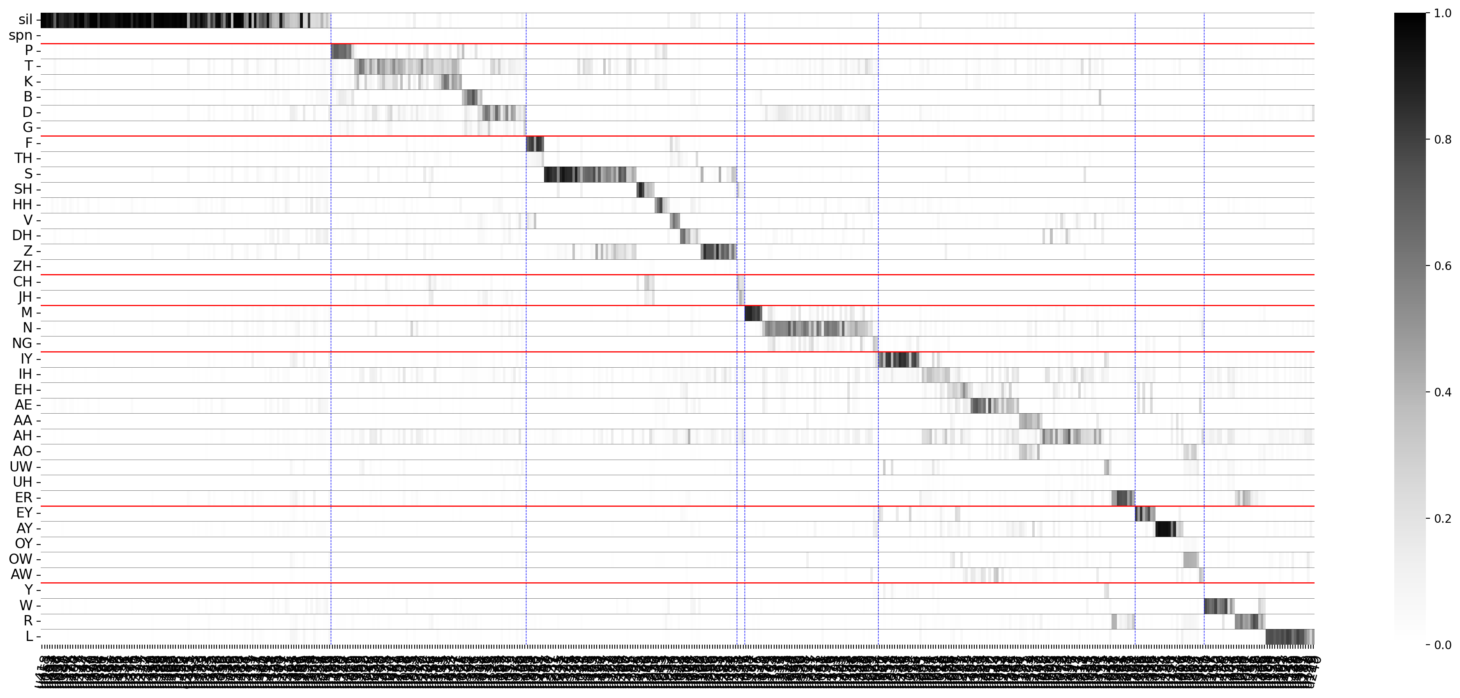
\includegraphics[width=\tempwidth]{feasiblefigs/ch4figs/hub-u050-ap0500-givenunit-byphn.png}
                 \caption{500 種次詞單位}
                 \label{fig:hub-u050-ap0500-givenunit-byphn}
             \end{subfigure}
             \vfill
             \begin{subfigure}{\textwidth}
                 \centering
                 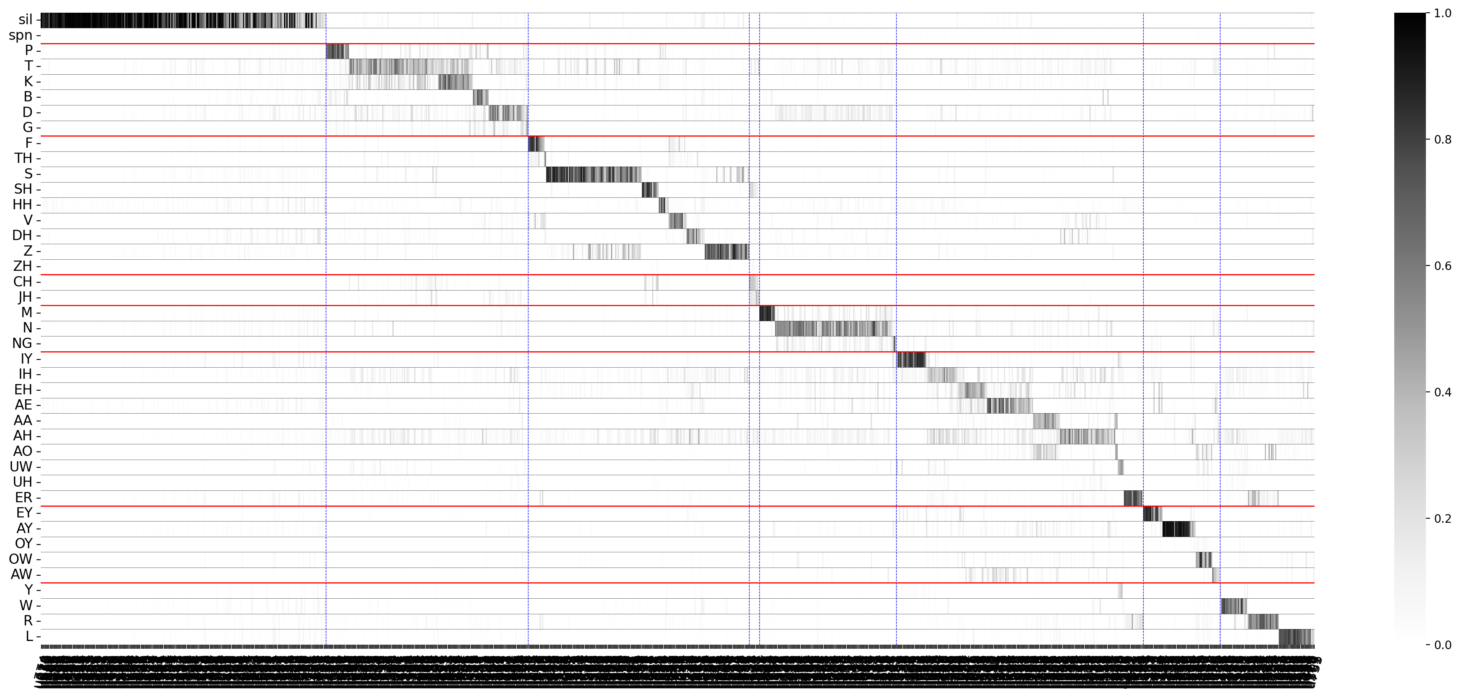
\includegraphics[width=\tempwidth]{feasiblefigs/ch4figs/hub-u050-ap1000-givenunit-byphn.png}
                 \caption{1000 種次詞單位}
                 \label{fig:hub-u050-ap1000-givenunit-byphn}
             \end{subfigure}

             \caption{HuBERT 表徵在 K-平均演算法使用分群數 50 後,}
             比較不同次詞單位數量的條件機率分佈 $p_{y|z}(i | j)$ 熱圖
             \label{fig:hub-u050-comparisons}
        \end{figure}
    }
    {
        \newcommand{\tempwidth}[0]{0.8\linewidth}
        \begin{figure}
             \centering
             \begin{subfigure}{\textwidth}
                 \centering
                 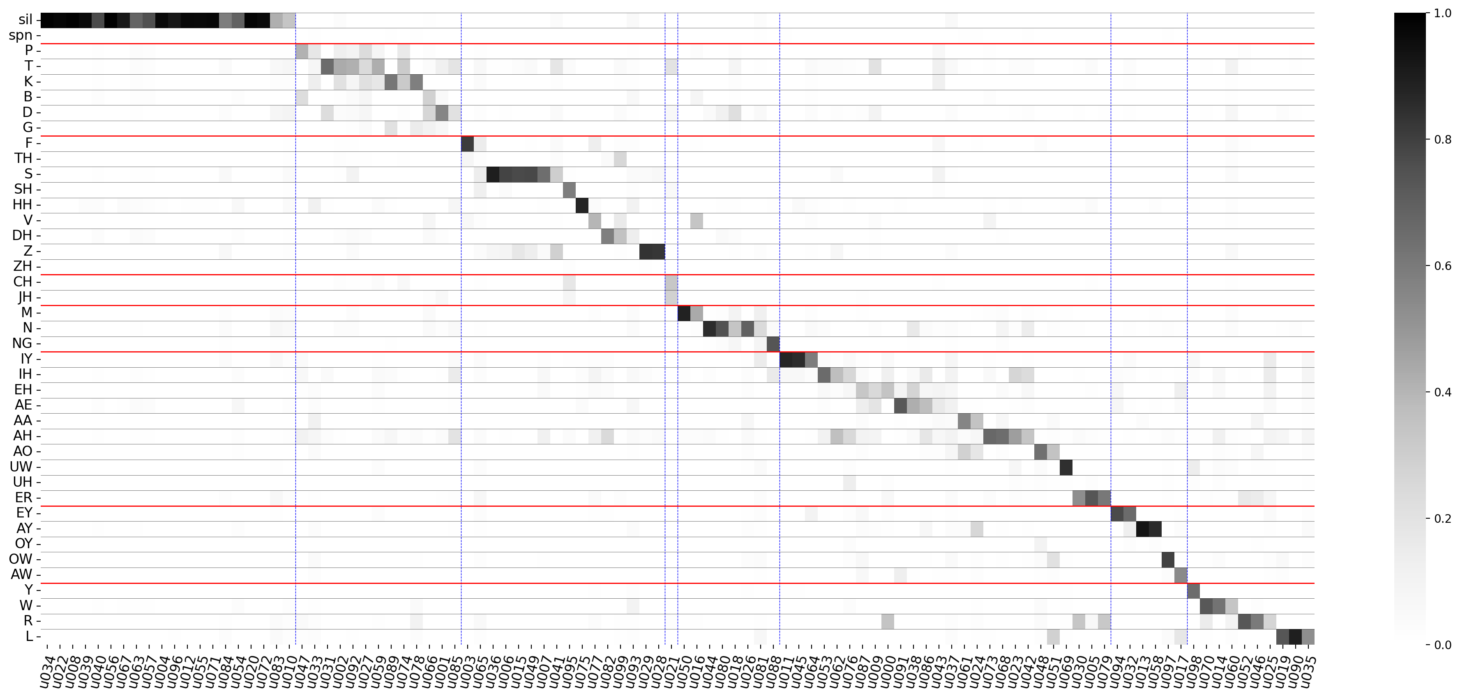
\includegraphics[width=\tempwidth]{feasiblefigs/ch4figs/hub-u100-ap0000-givenunit-byphn.png}
                 \caption{離散單元}
                 \label{fig:hub-u100-ap0000-givenunit-byphn}
             \end{subfigure}
             \vfill
             \begin{subfigure}{\textwidth}
                 \centering
                 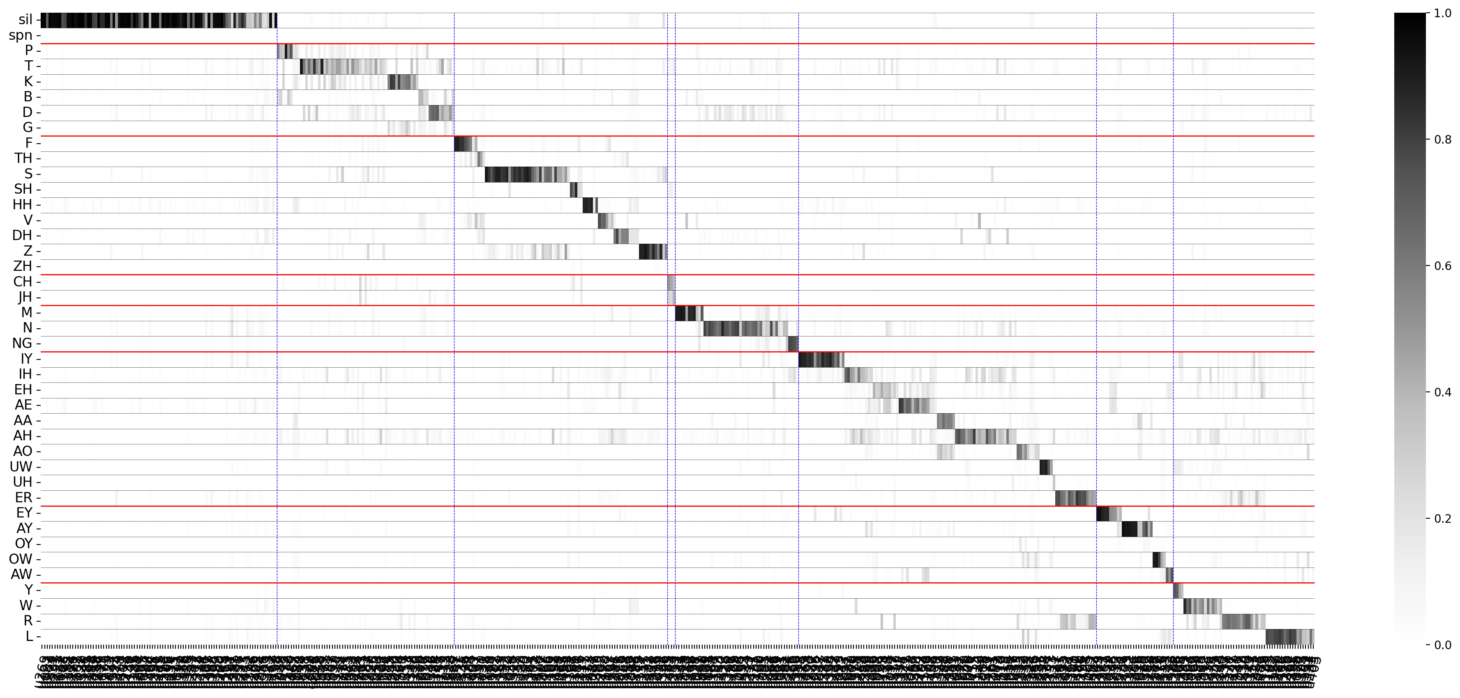
\includegraphics[width=\tempwidth]{feasiblefigs/ch4figs/hub-u100-ap0500-givenunit-byphn.png}
                 \caption{500 種次詞單位}
                 \label{fig:hub-u100-ap0500-givenunit-byphn}
             \end{subfigure}
             \vfill
             \begin{subfigure}{\textwidth}
                 \centering
                 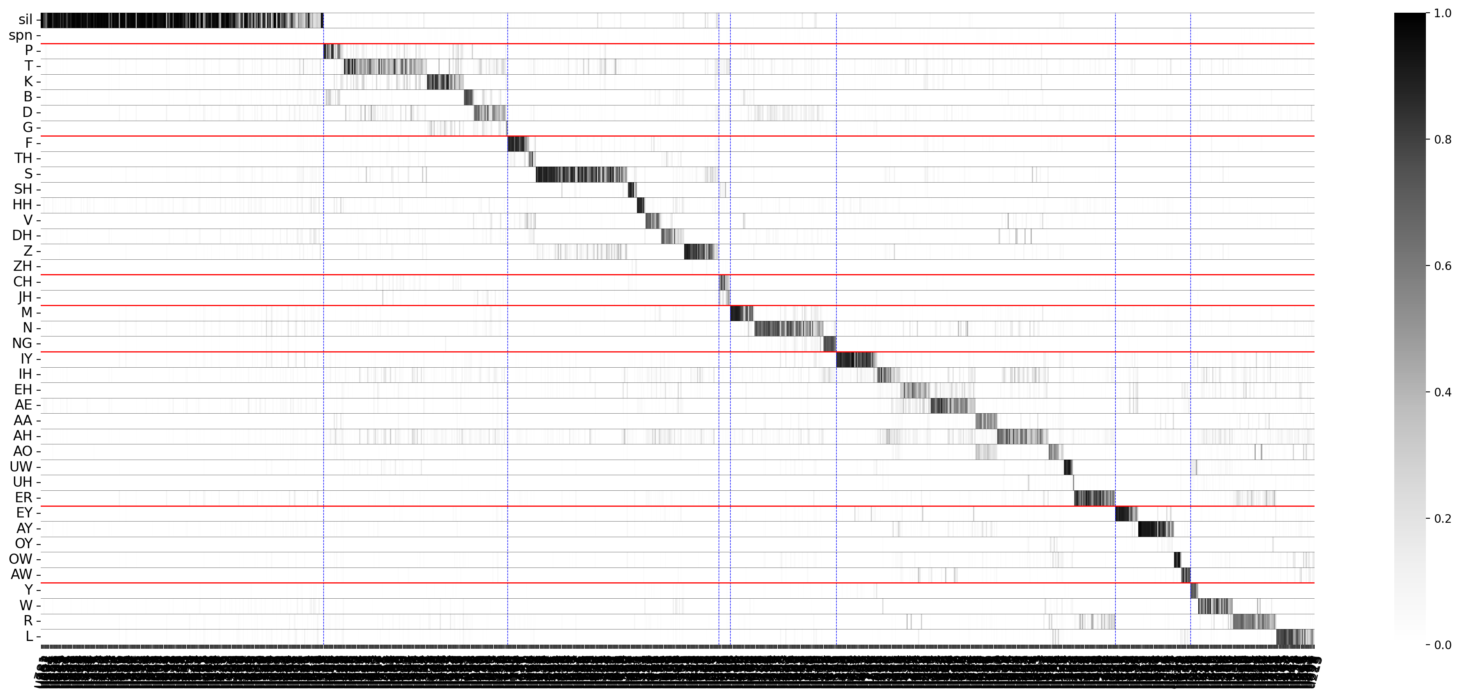
\includegraphics[width=\tempwidth]{feasiblefigs/ch4figs/hub-u100-ap1000-givenunit-byphn.png}
                 \caption{1000 種次詞單位}
                 \label{fig:hub-u100-ap1000-givenunit-byphn}
             \end{subfigure}

             \caption{HuBERT 表徵在 K-平均演算法使用分群數 100 後,}
             比較不同次詞單位數量的條件機率分佈 $p_{y|z}(i | j)$ 熱圖
             \label{fig:hub-u100-comparisons}
        \end{figure}
    }
}

{
    {
        \newcommand{\tempwidth}[0]{0.7\linewidth}
        \begin{figure}
             \centering
             \begin{subfigure}{\textwidth}
                 \centering
                 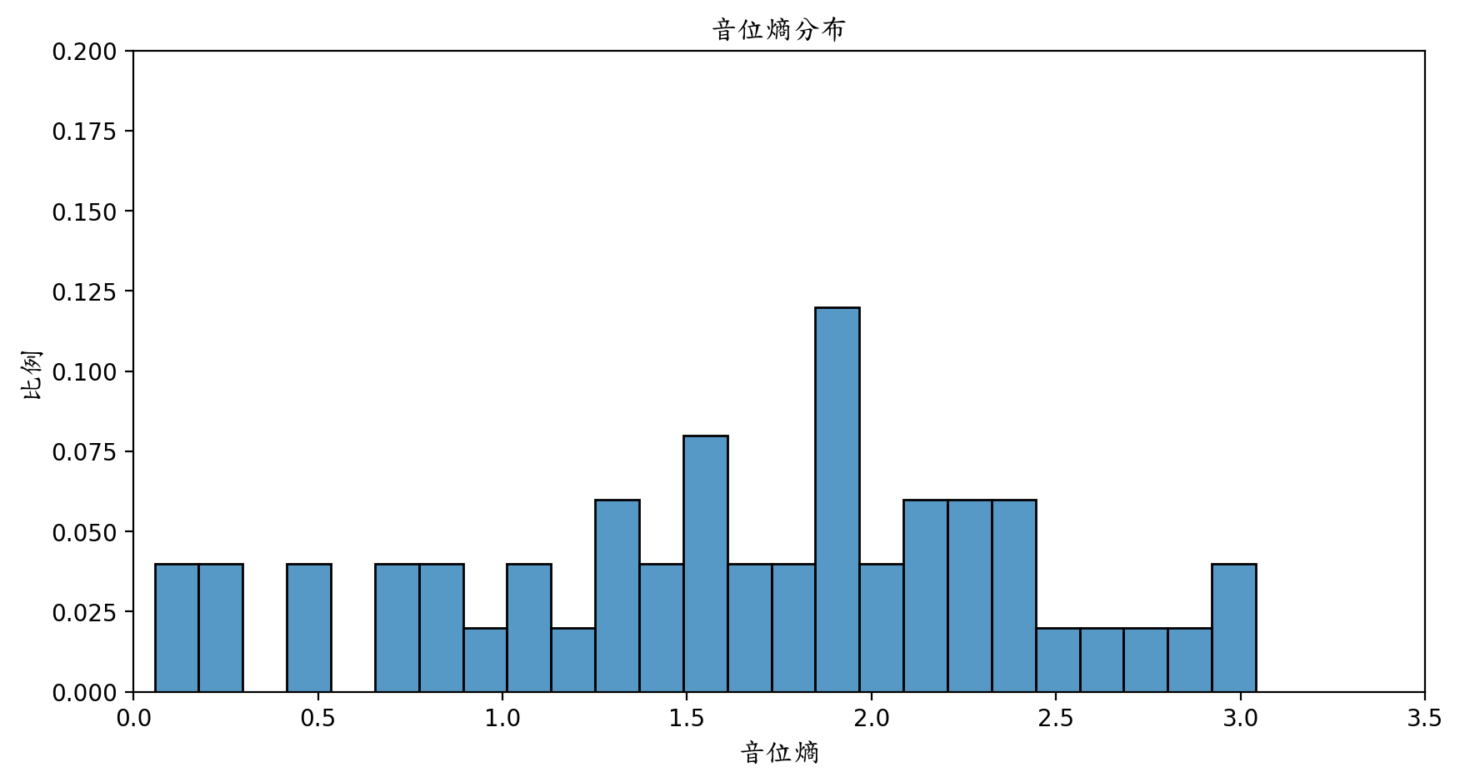
\includegraphics[width=\tempwidth]{feasiblefigs/ch4figs/hub-u050-ap0000-phnent-hist.png}
                 \caption{離散單元}
                 \label{fig:hub-u050-ap0000-phnent-hist}
             \end{subfigure}
             \vfill
             \begin{subfigure}{\textwidth}
                 \centering
                 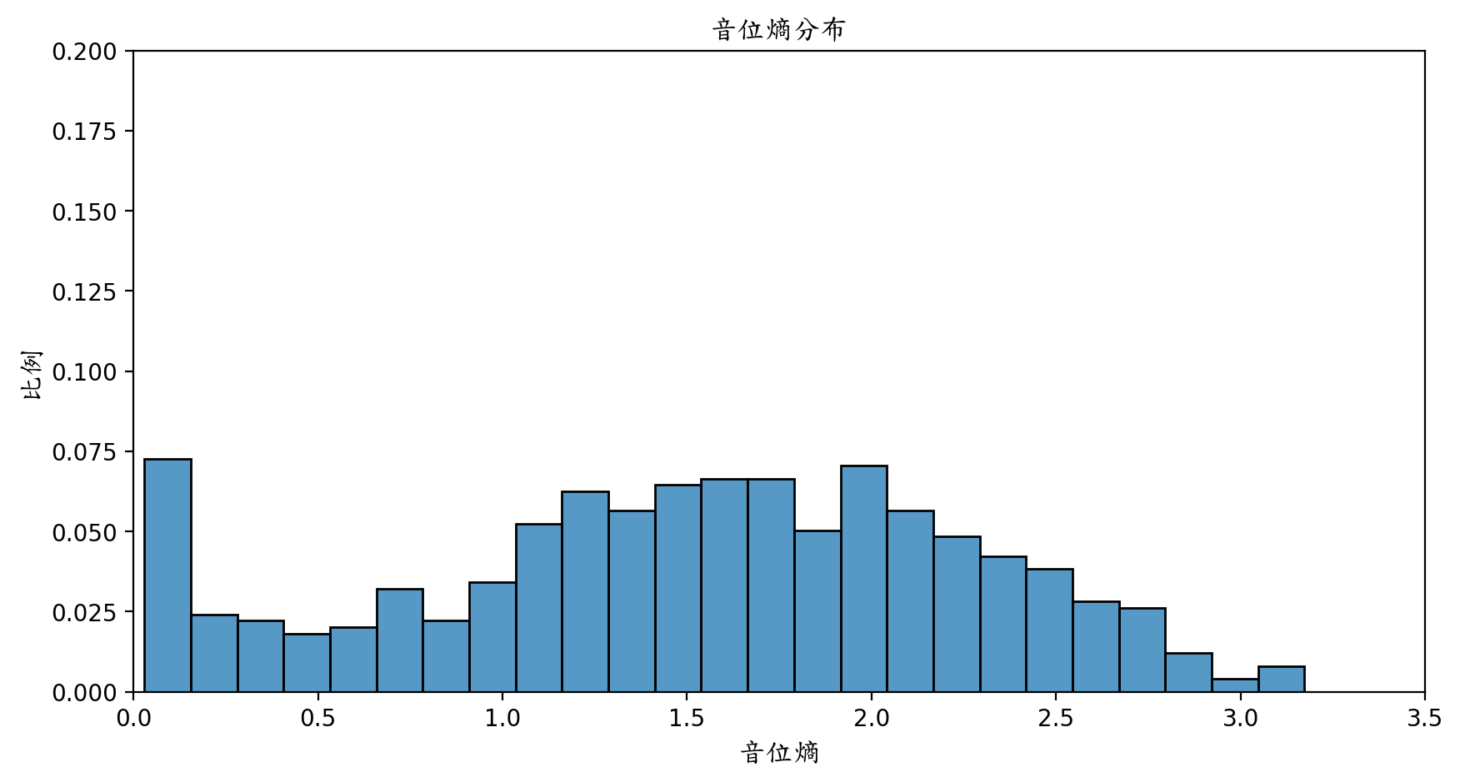
\includegraphics[width=\tempwidth]{feasiblefigs/ch4figs/hub-u050-ap0500-phnent-hist.png}
                 \caption{500 種次詞單位}
                 \label{fig:hub-u050-ap0500-phnent-hist}
             \end{subfigure}
             \vfill
             \begin{subfigure}{\textwidth}
                 \centering
                 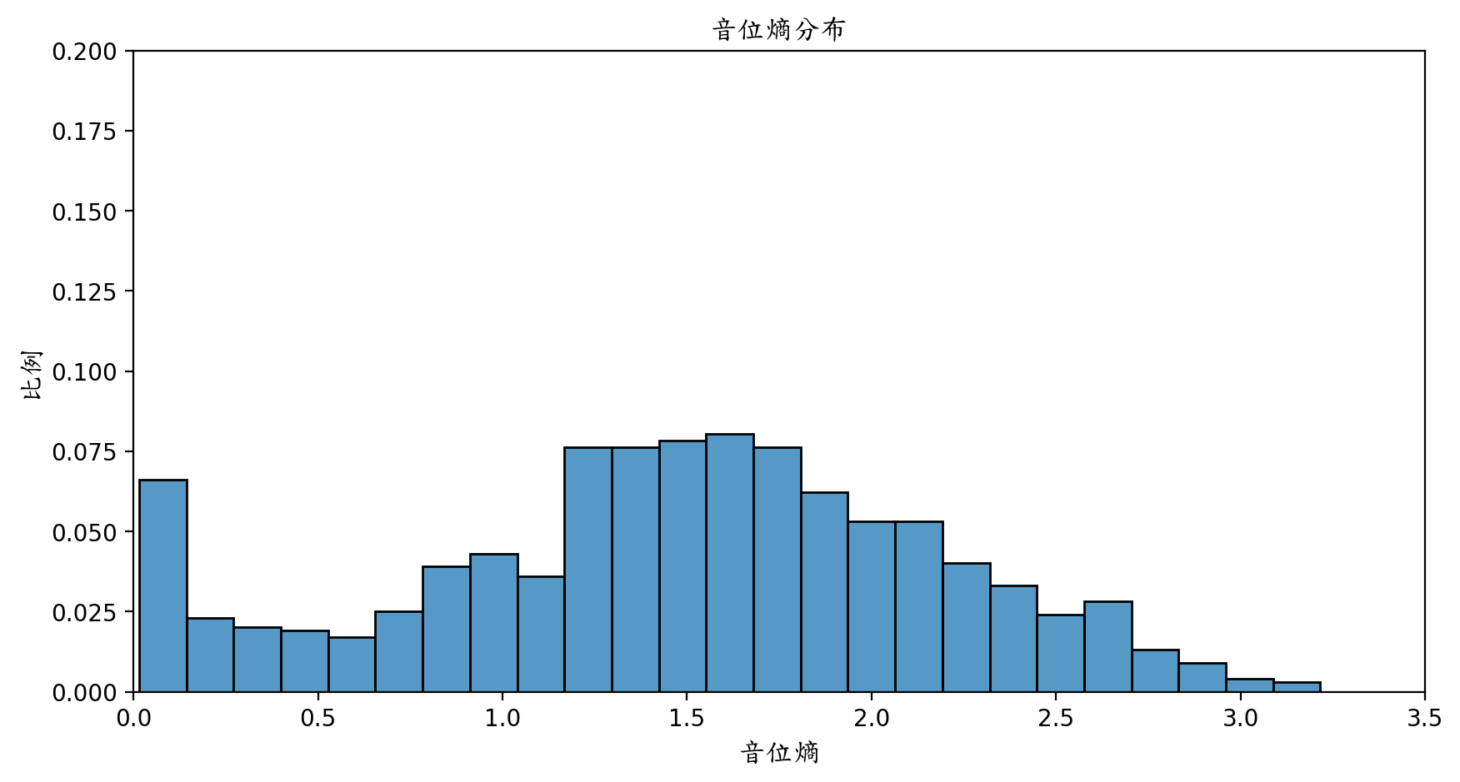
\includegraphics[width=\tempwidth]{feasiblefigs/ch4figs/hub-u050-ap1000-phnent-hist.png}
                 \caption{1000 種次詞單位}
                 \label{fig:hub-u050-ap1000-phnent-hist}
             \end{subfigure}

             \caption{HuBERT 表徵在 K-平均演算法使用分群數 50 後,}
             比較不同次詞單位數量的條音位條件熵 $H(y|z)$ 直方圖
             \label{fig:hub-u050-hist-comparisons}
        \end{figure}
    }
    {
        \newcommand{\tempwidth}[0]{0.7\linewidth}
        \begin{figure}
             \centering
             \begin{subfigure}{\textwidth}
                 \centering
                 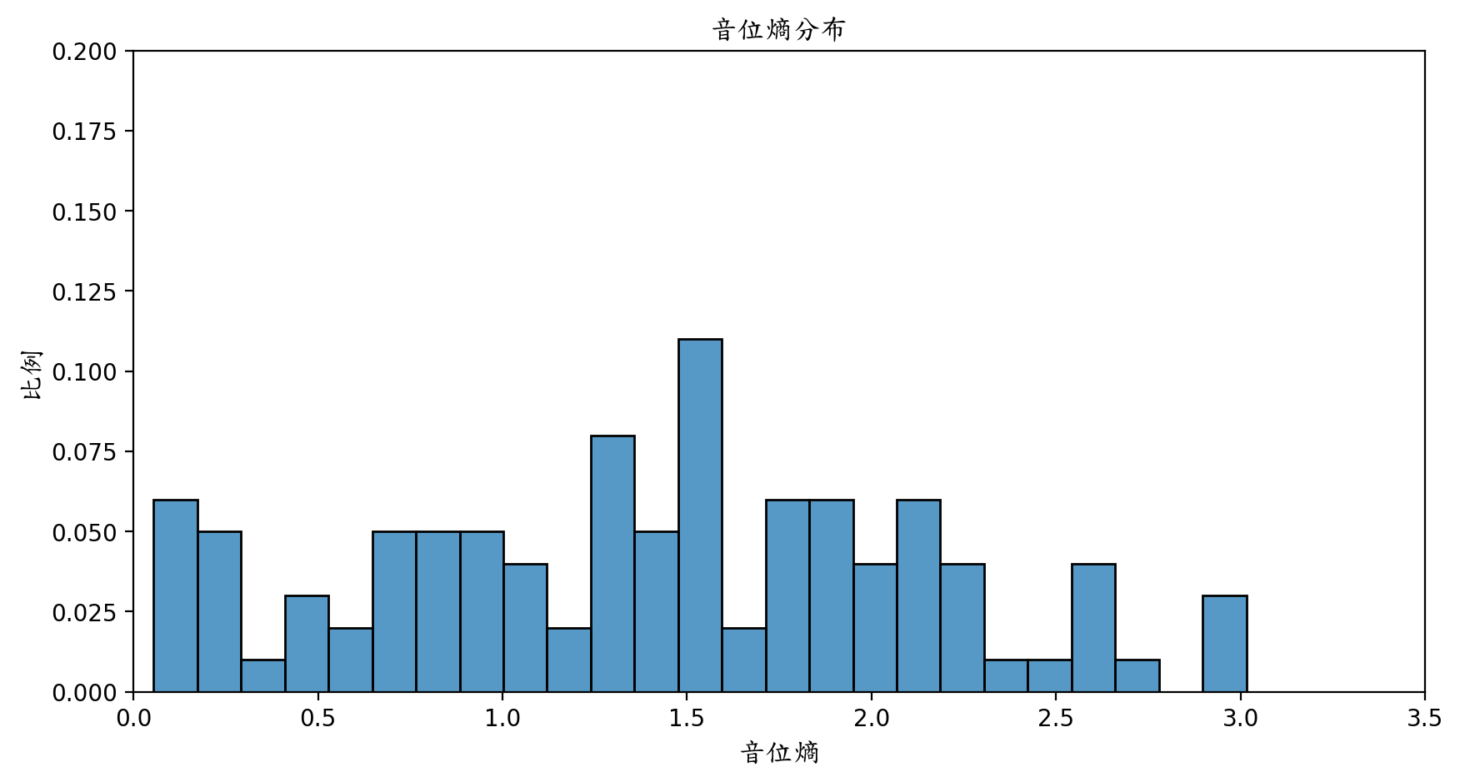
\includegraphics[width=\tempwidth]{feasiblefigs/ch4figs/hub-u100-ap0000-phnent-hist.png}
                 \caption{離散單元}
                 \label{fig:hub-u100-ap0000-phnent-hist}
             \end{subfigure}
             \vfill
             \begin{subfigure}{\textwidth}
                 \centering
                 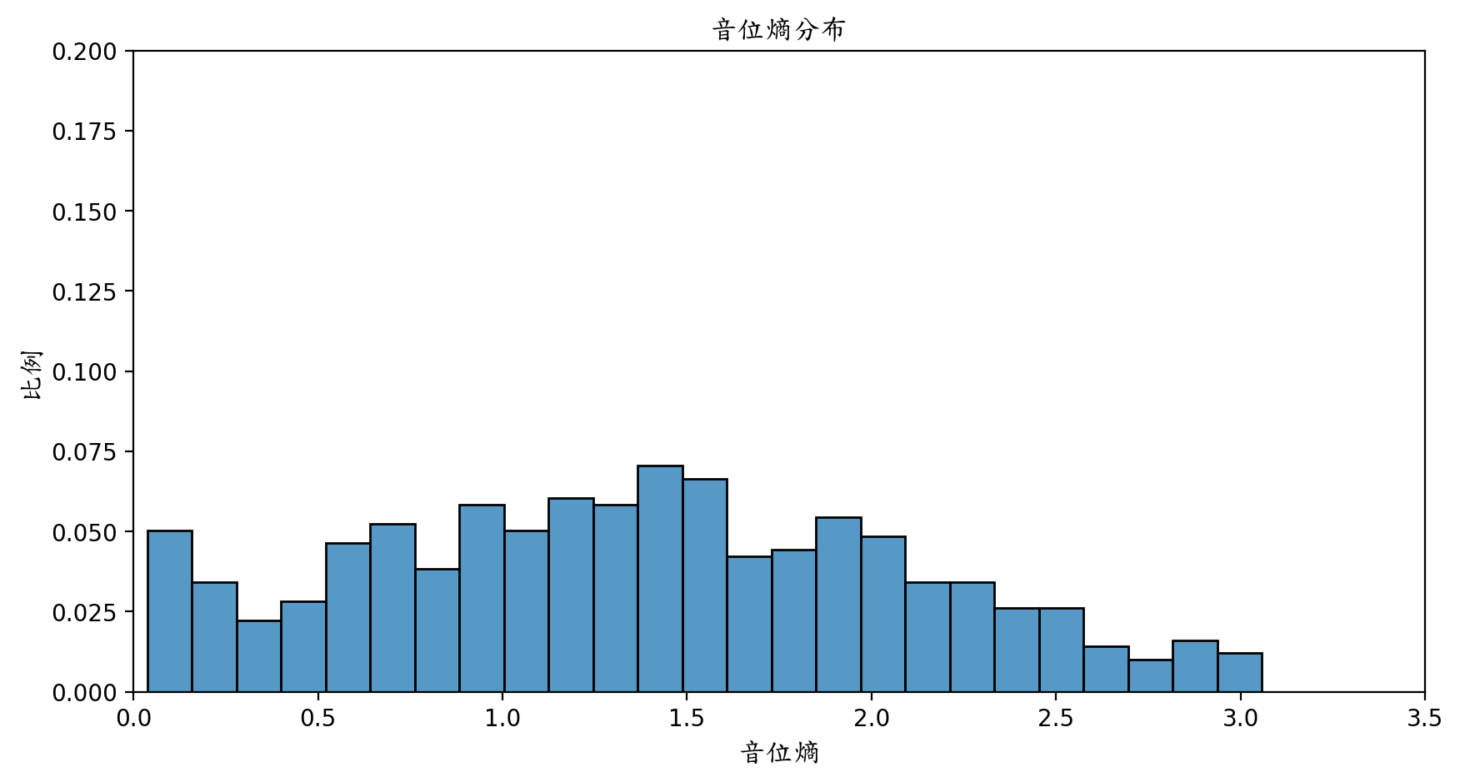
\includegraphics[width=\tempwidth]{feasiblefigs/ch4figs/hub-u100-ap0500-phnent-hist.png}
                 \caption{500 種次詞單位}
                 \label{fig:hub-u100-ap0500-phnent-hist}
             \end{subfigure}
             \vfill
             \begin{subfigure}{\textwidth}
                 \centering
                 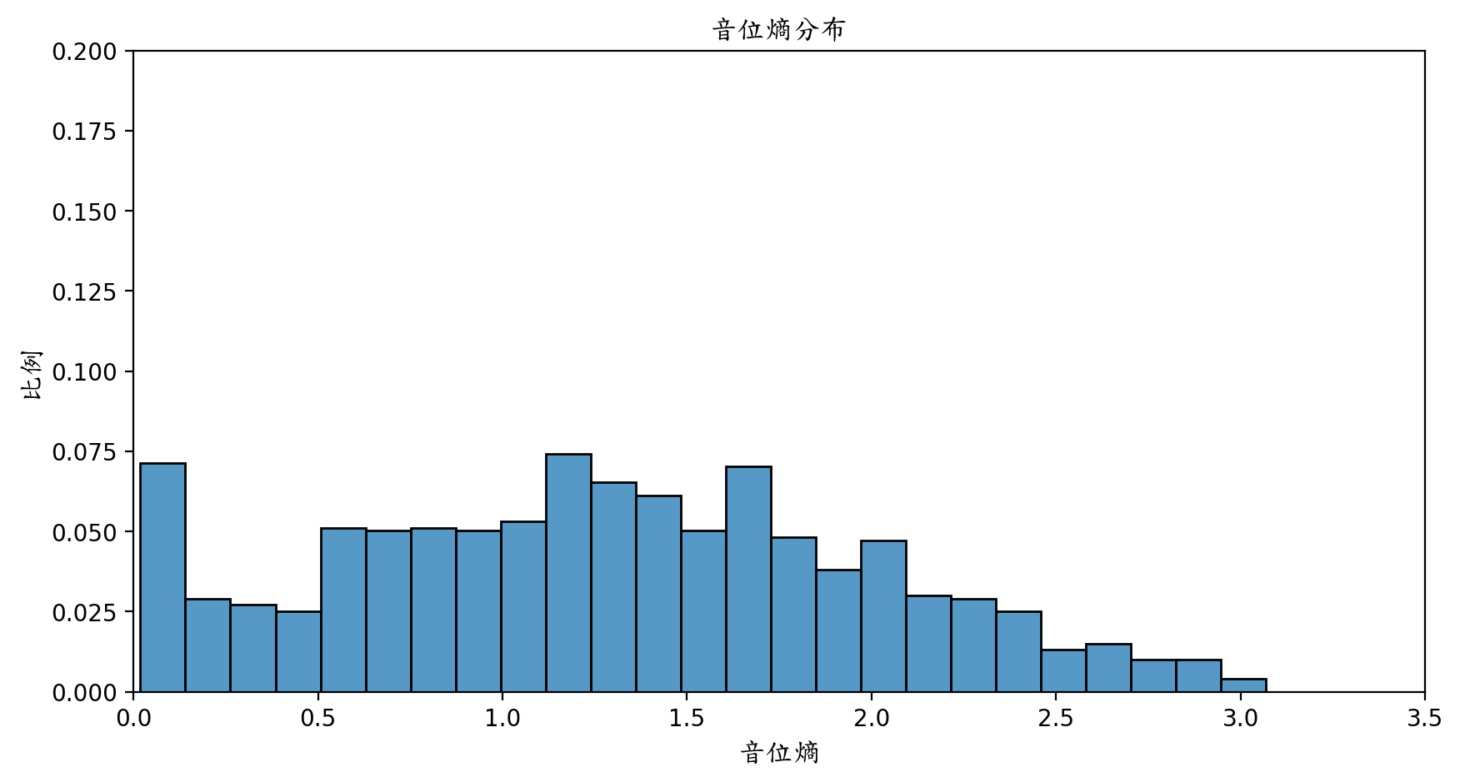
\includegraphics[width=\tempwidth]{feasiblefigs/ch4figs/hub-u100-ap1000-phnent-hist.png}
                 \caption{1000 種次詞單位}
                 \label{fig:hub-u100-ap1000-phnent-hist}
             \end{subfigure}

             \caption{HuBERT 表徵在 K-平均演算法使用分群數 100 後,}
             比較不同次詞單位數量的音位條件熵 $H(y|z)$ 直方圖
             \label{fig:hub-u100-hist-comparisons}
        \end{figure}
    }
}


  首先,為了觀察聲學片段數量對於機率熱圖與純度數據的影響,圖 \ref{fig:hub-u050-comparisons} 與圖 \ref{fig:hub-u100-comparisons} 分別以
 HuBERT 模型分群數為 50 和 100 為基礎,
比較了不同聲學片段數量的條件機率熱圖。
% 它們分別是 HuBERT 模型配合分群數為 50 和 100 的離散單元模型,並將各自的離散單元使用單一詞演算法得到次詞單位數量為 500 和 1000 的聲學片段所得到的結果。\par

        從中我們可以看出,當聲學片段數量上升時,由於有了更多的符記可以讓離散表徵區別更細節的發音差異,因此整體的純度數值有所提升。從熱圖上也可以觀察出更深的色塊,也就是有了更多的符記可以集中的對應到特定音位。然而,由於符記數量的上升,機率熱圖整體也變得更加碎片化,因此歸類同樣音位的效果也相對變得較不明顯。\par
        為了確認每個聲學片段對應音位之集中狀況,我們可以觀察音位熵的直方圖變化。一樣比較 HuBERT 模型、K-平均分群數 50 和 100 在使用 500 和 1000 個次詞單位得到的聲學片段所對應的音位條件熵 $H(y|z)$ 的直方圖,呈現在圖 \ref{fig:hub-u050-hist-comparisons} 與圖 \ref{fig:hub-u100-hist-comparisons} 中,可以看出,透過分詞方法的引入,相比於尚未使用的單一離散單元進行的統計數據,改用聲學片段可以讓整體的音位熵確實降低,亦即各自符記對應的音位變得更加明確,與我們從機率熱圖上所觀察到的趨勢符合。\par
        雖然改用聲學片段會使熱圖的對應規律變得更加複雜而難以觀察,但除純度與相互資訊的數值變化外,從符記代表性音位的比例變化,也可以驗證更多的符記可以區別發音細節這點。我們回到圖 \ref{fig:hub-u050-comparisons} 中觀察 HuBERT 在分群數 50 時的機率熱圖,圖中的藍色鉛直線是每個聲學片段按對應音位之分類,排序分區的結果。因此觀察藍色鉛直線在橫軸上各區的比例變化,可以理解這些符記以多少的比例對應不同音位的發音特徵。第三章在單一離散單元分群數為 50 時,由於離散單元數較少,並沒有任何單元最高機率對應塞擦音音位。然而,當對這些離散單元進行分詞處理後,不管在次詞單位數量為 500 或 1000 的機率熱圖上,都可以看見出現了至少一個符記可以對應到塞擦音,由此驗證藉由引入分詞方法提升次詞單位數量,對捕捉更細微的發音差異的確是有所幫助的。


\subsubsection{原先離散單元分群數對聲學片段的影響}


{
    {
        \begin{figure}
             \centering
             \begin{subfigure}{\textwidth}
                 \centering
                 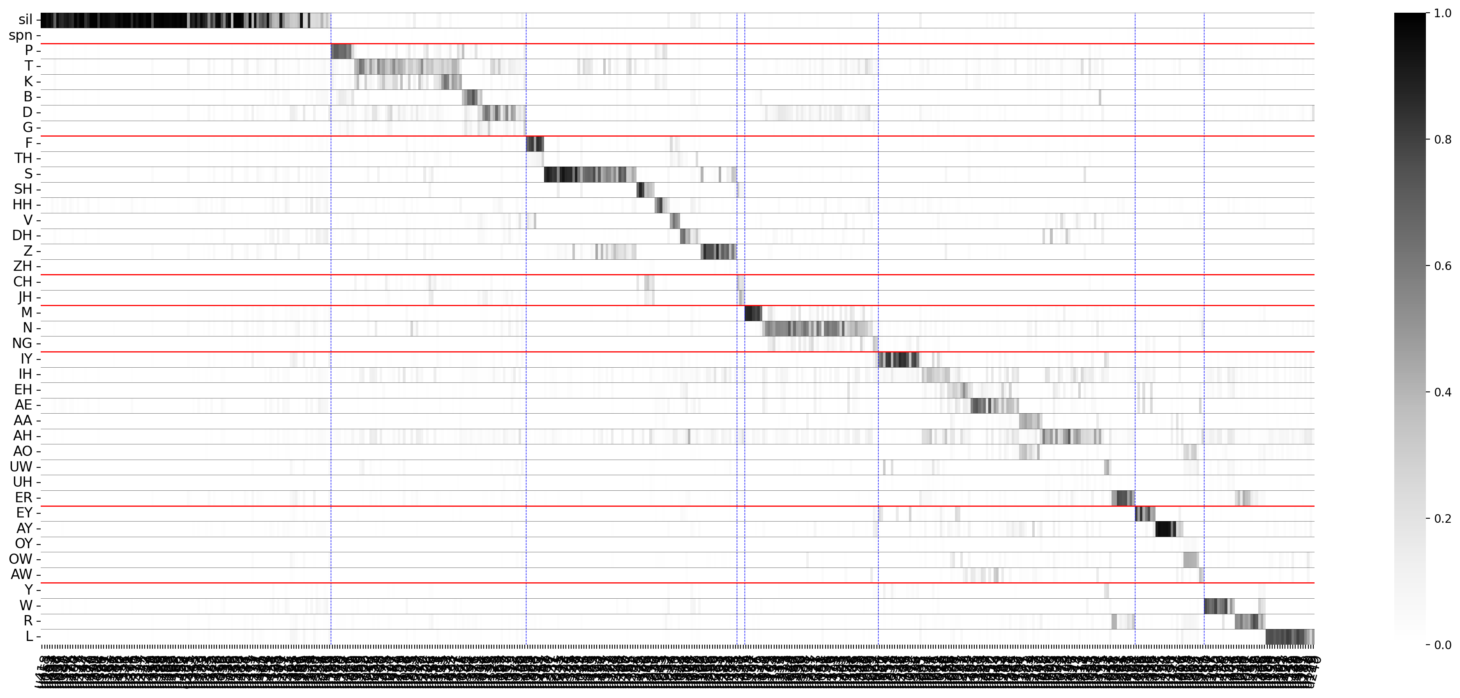
\includegraphics[width=1\linewidth]{feasiblefigs/ch4figs/hub-u050-ap0500-givenunit-byphn.png}
                 \caption{分群數 50}
                 \label{fig:hub-u050-ap0500-givenunit-byphn--picked}
             \end{subfigure}
             \vfill
             \begin{subfigure}{\textwidth}
                 \centering
                 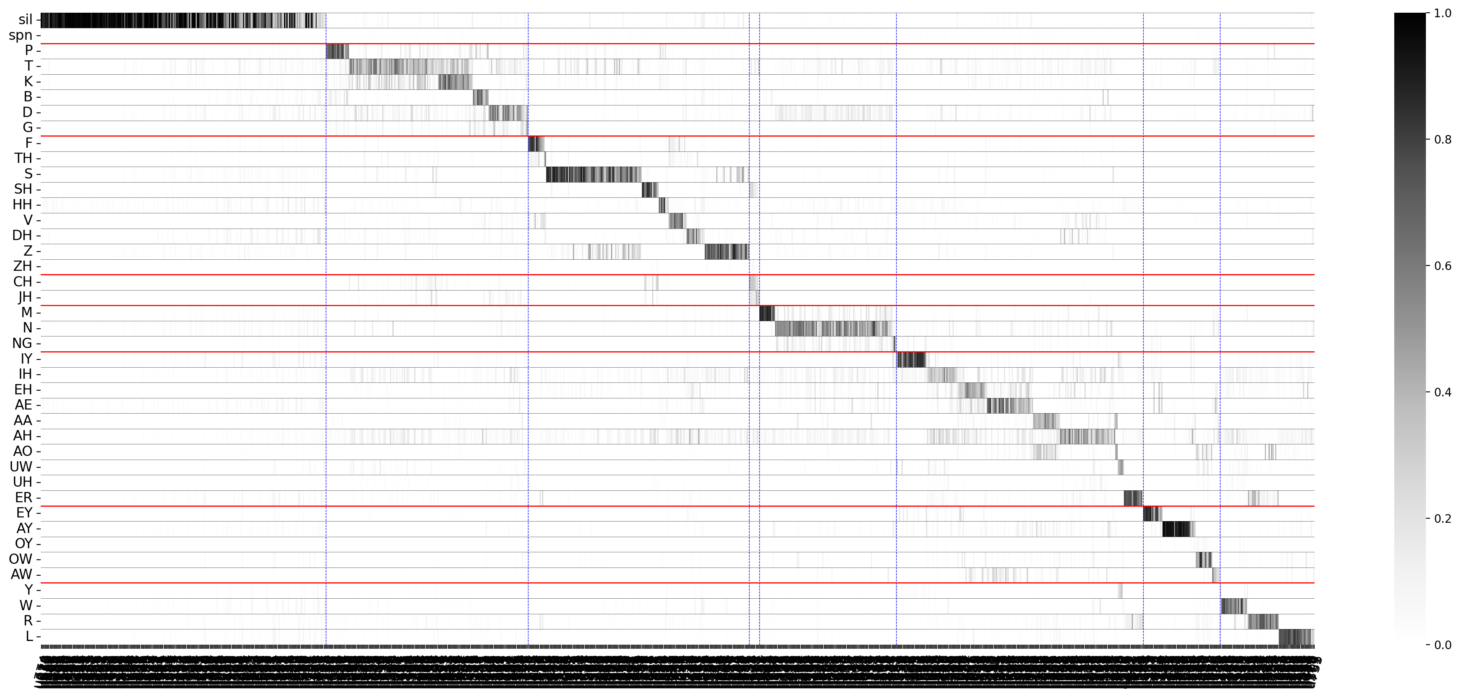
\includegraphics[width=1\linewidth]{feasiblefigs/ch4figs/hub-u050-ap1000-givenunit-byphn.png}
                 \caption{分群數 100}
                 \label{fig:hub-u100-ap0500-givenunit-byphn--picked}
             \end{subfigure}
             \caption{比較同樣 500 種次詞單位的聲學片段模型,著重比較 HuBERT 表徵}
             在 K-平均演算法使用分群數 50 與 100 的條件機率熱圖 $p_{y|z}(i|j)$ 差異
             \label{fig:check-ap0500}
        \end{figure}
    }
}



  然而,儘管分詞方法的引入在一定程度上幫助了區別語音訊號中的細微發音差異,若要更直接的對這件事進行改善,在原始的語音表徵進行 K-平均演算法離散化時,其分群數仍為了更關鍵的決定因素。圖 \ref{fig:check-ap0500} 比較了同樣次詞單位數量為 500 時,離散表徵分群數為 50 和 100 的機率熱圖差異,可以發現分群數為 100 的機率熱圖能更加平均的對應到不同的音位,而不如分群數 50 的機率熱圖對於某些音位的捕捉效果那麼不平均。然而,即便對音位標註的歸類效果最大的取決於離散單元分群數,在遇到運算資源限制,使得使用大量分群數進行 K-平均演算法難以實行時,仍舊可以藉助分詞方法的引入提升整體表現。
        \jcm{藉由比較幾章機率熱圖的差異,我們可以確認這件事。 \jcm{補寫一下}}

        \jcm{
        
        我們這邊可以比較一下 50、100、50+100、50+500、100+500 的熱圖。從這邊可以驗證前面所說的:在基底分群數確定的情形之下,的確一開始分群數開得比較大,整體對語音規律的捕捉效果就會比較好,但藉由分群方法的引入,至少 50 分群數可以藉由符記數提升的機會,來重新編碼語音中的結構,也就是雖然不如 K-平均演算法那樣因為直接做用於語音表徵空間,那麼好區分出發音的差異,但藉由分詞演算法,仍然可以從捕捉語音中明顯重複的序列資訊\textcolor{red}{[這時候是不是要擺一下長度 & 常見 pattern 統計數據確認了?] } ,獲取語音序列中跟發音有關的特徵,進而模擬類似人類理解音位的過程。
        
        }
}

    {
        \newcommand{\tempwidth}[0]{0.8\linewidth}
        \begin{figure}
             \centering
             \begin{subfigure}{\textwidth}
                 \centering
                 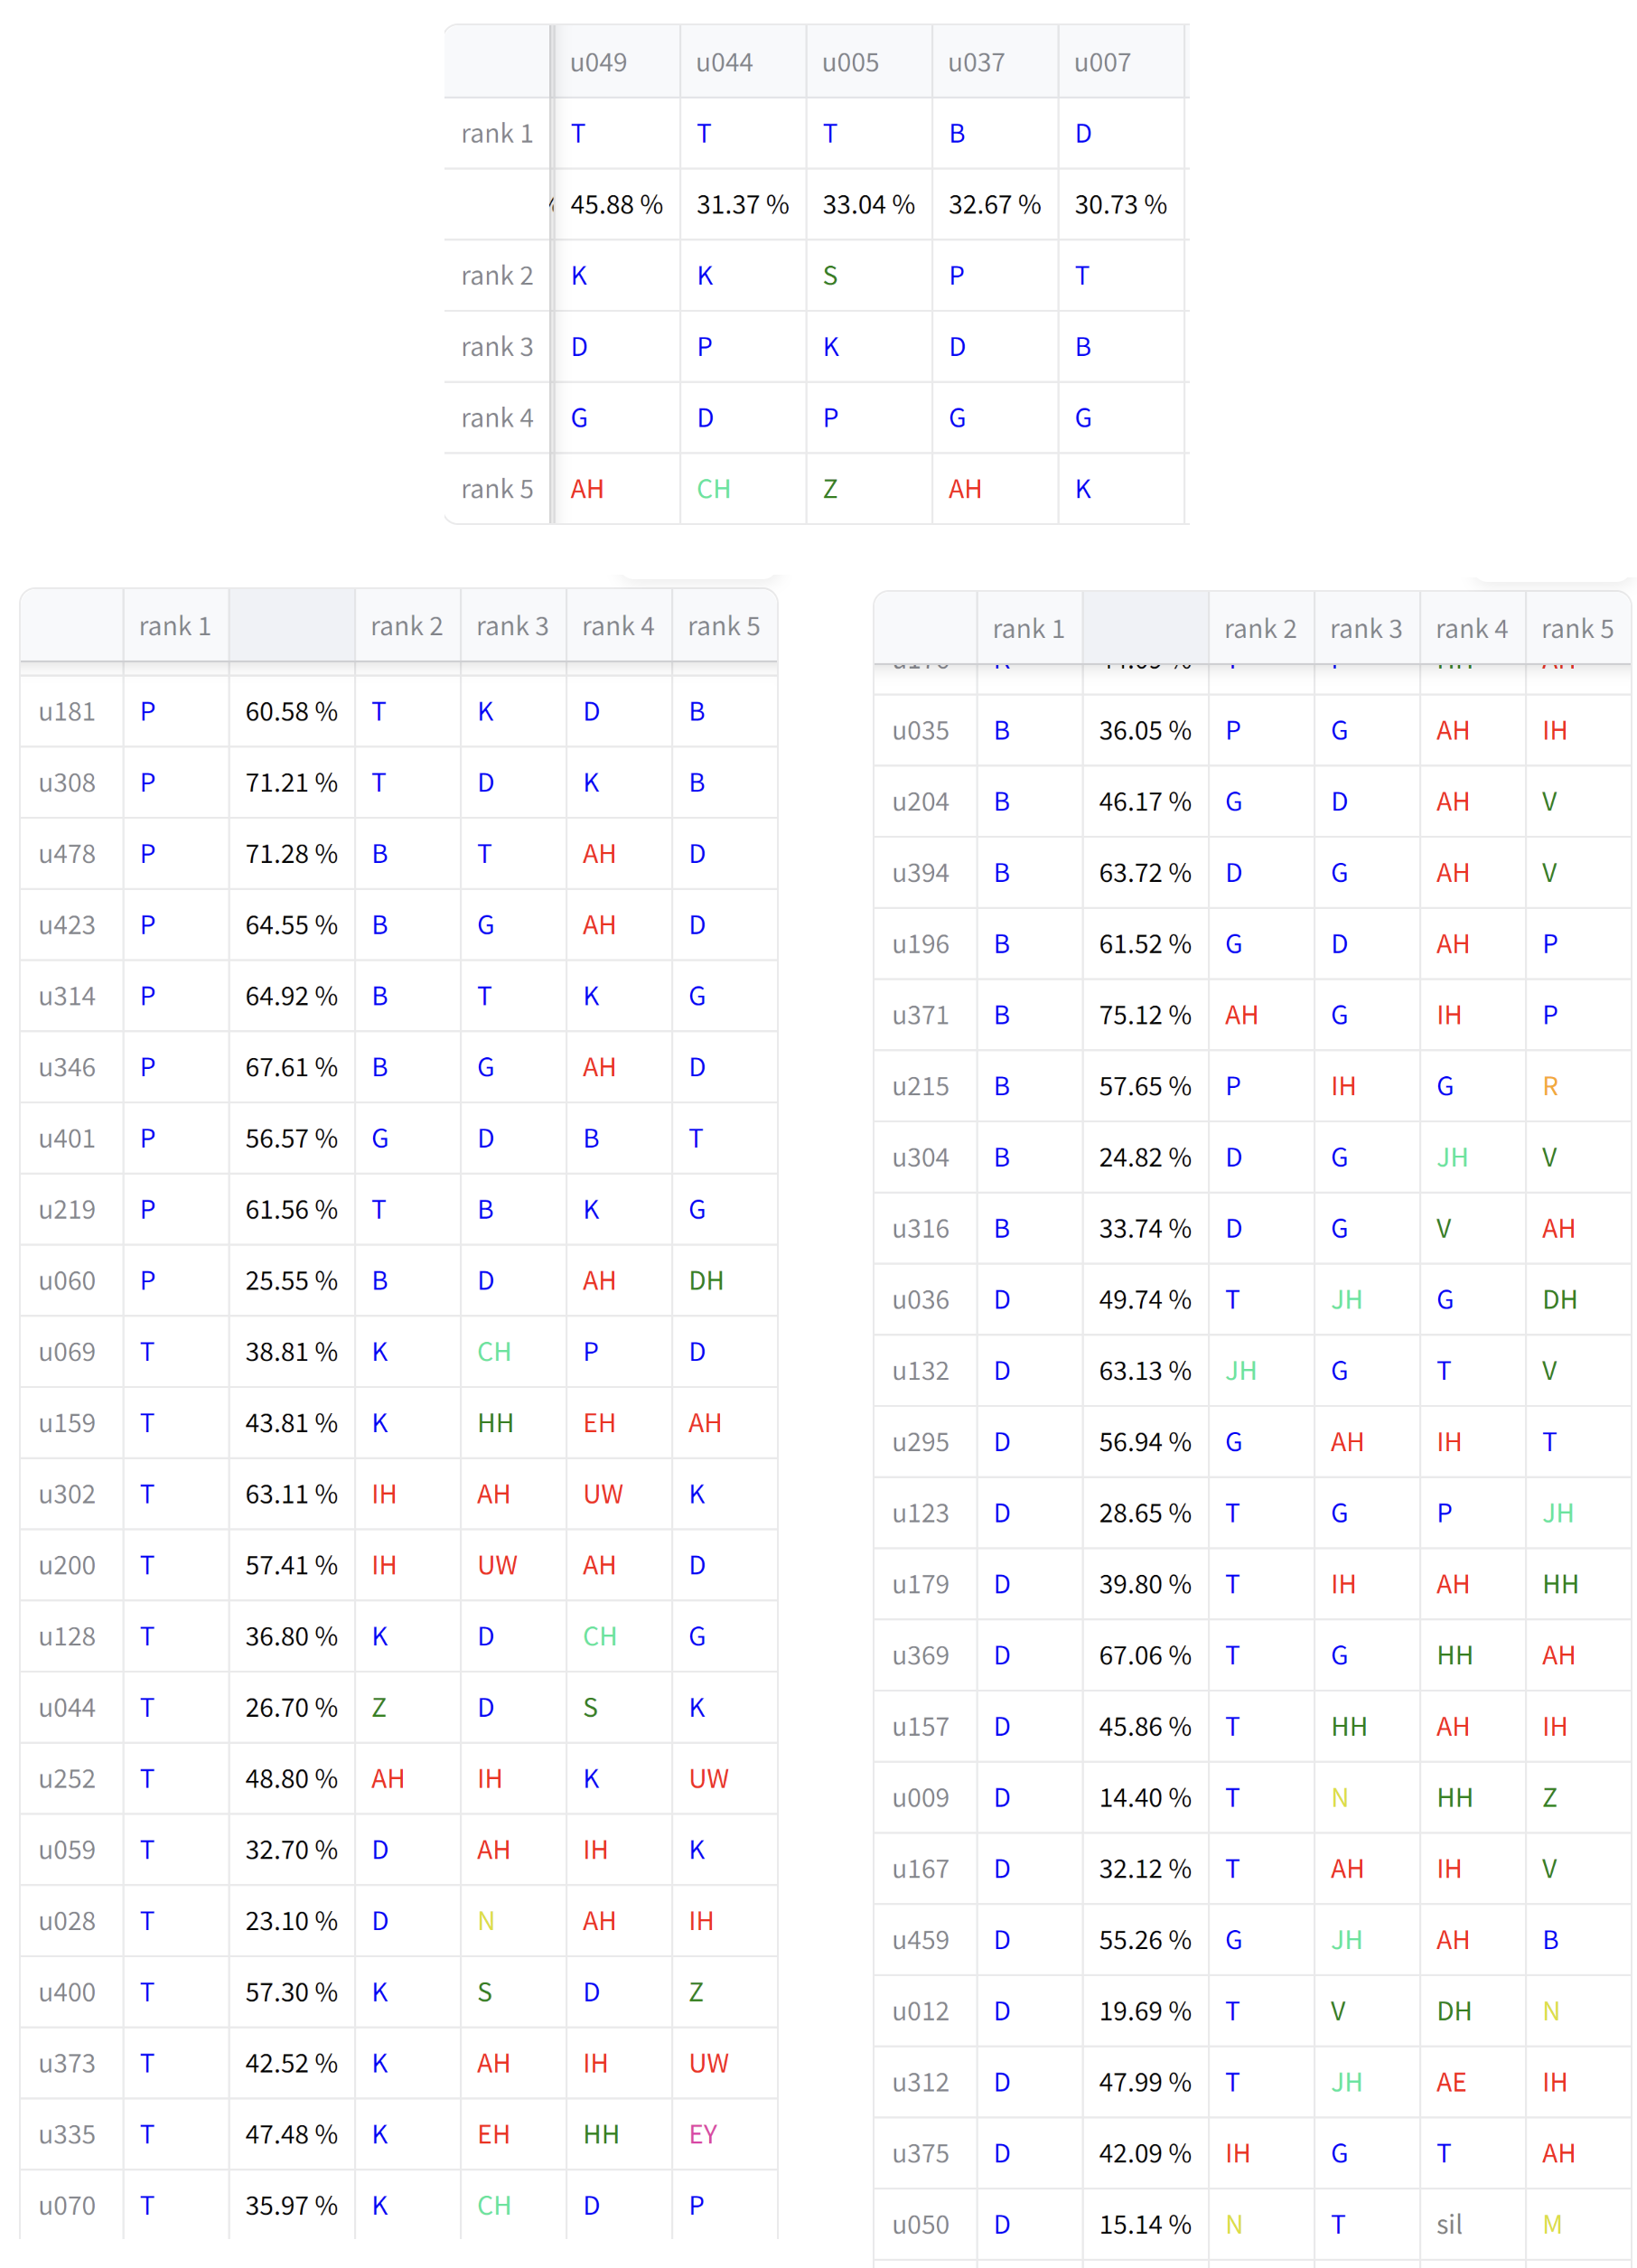
\includegraphics[width=\tempwidth]{chapters/plo_phn.png}
                 \caption{塞音}
                 \label{fig:hub-u050-ap0500-ploobs}
             \end{subfigure}
             \vfill
             \begin{subfigure}{\textwidth}
                 \centering
                 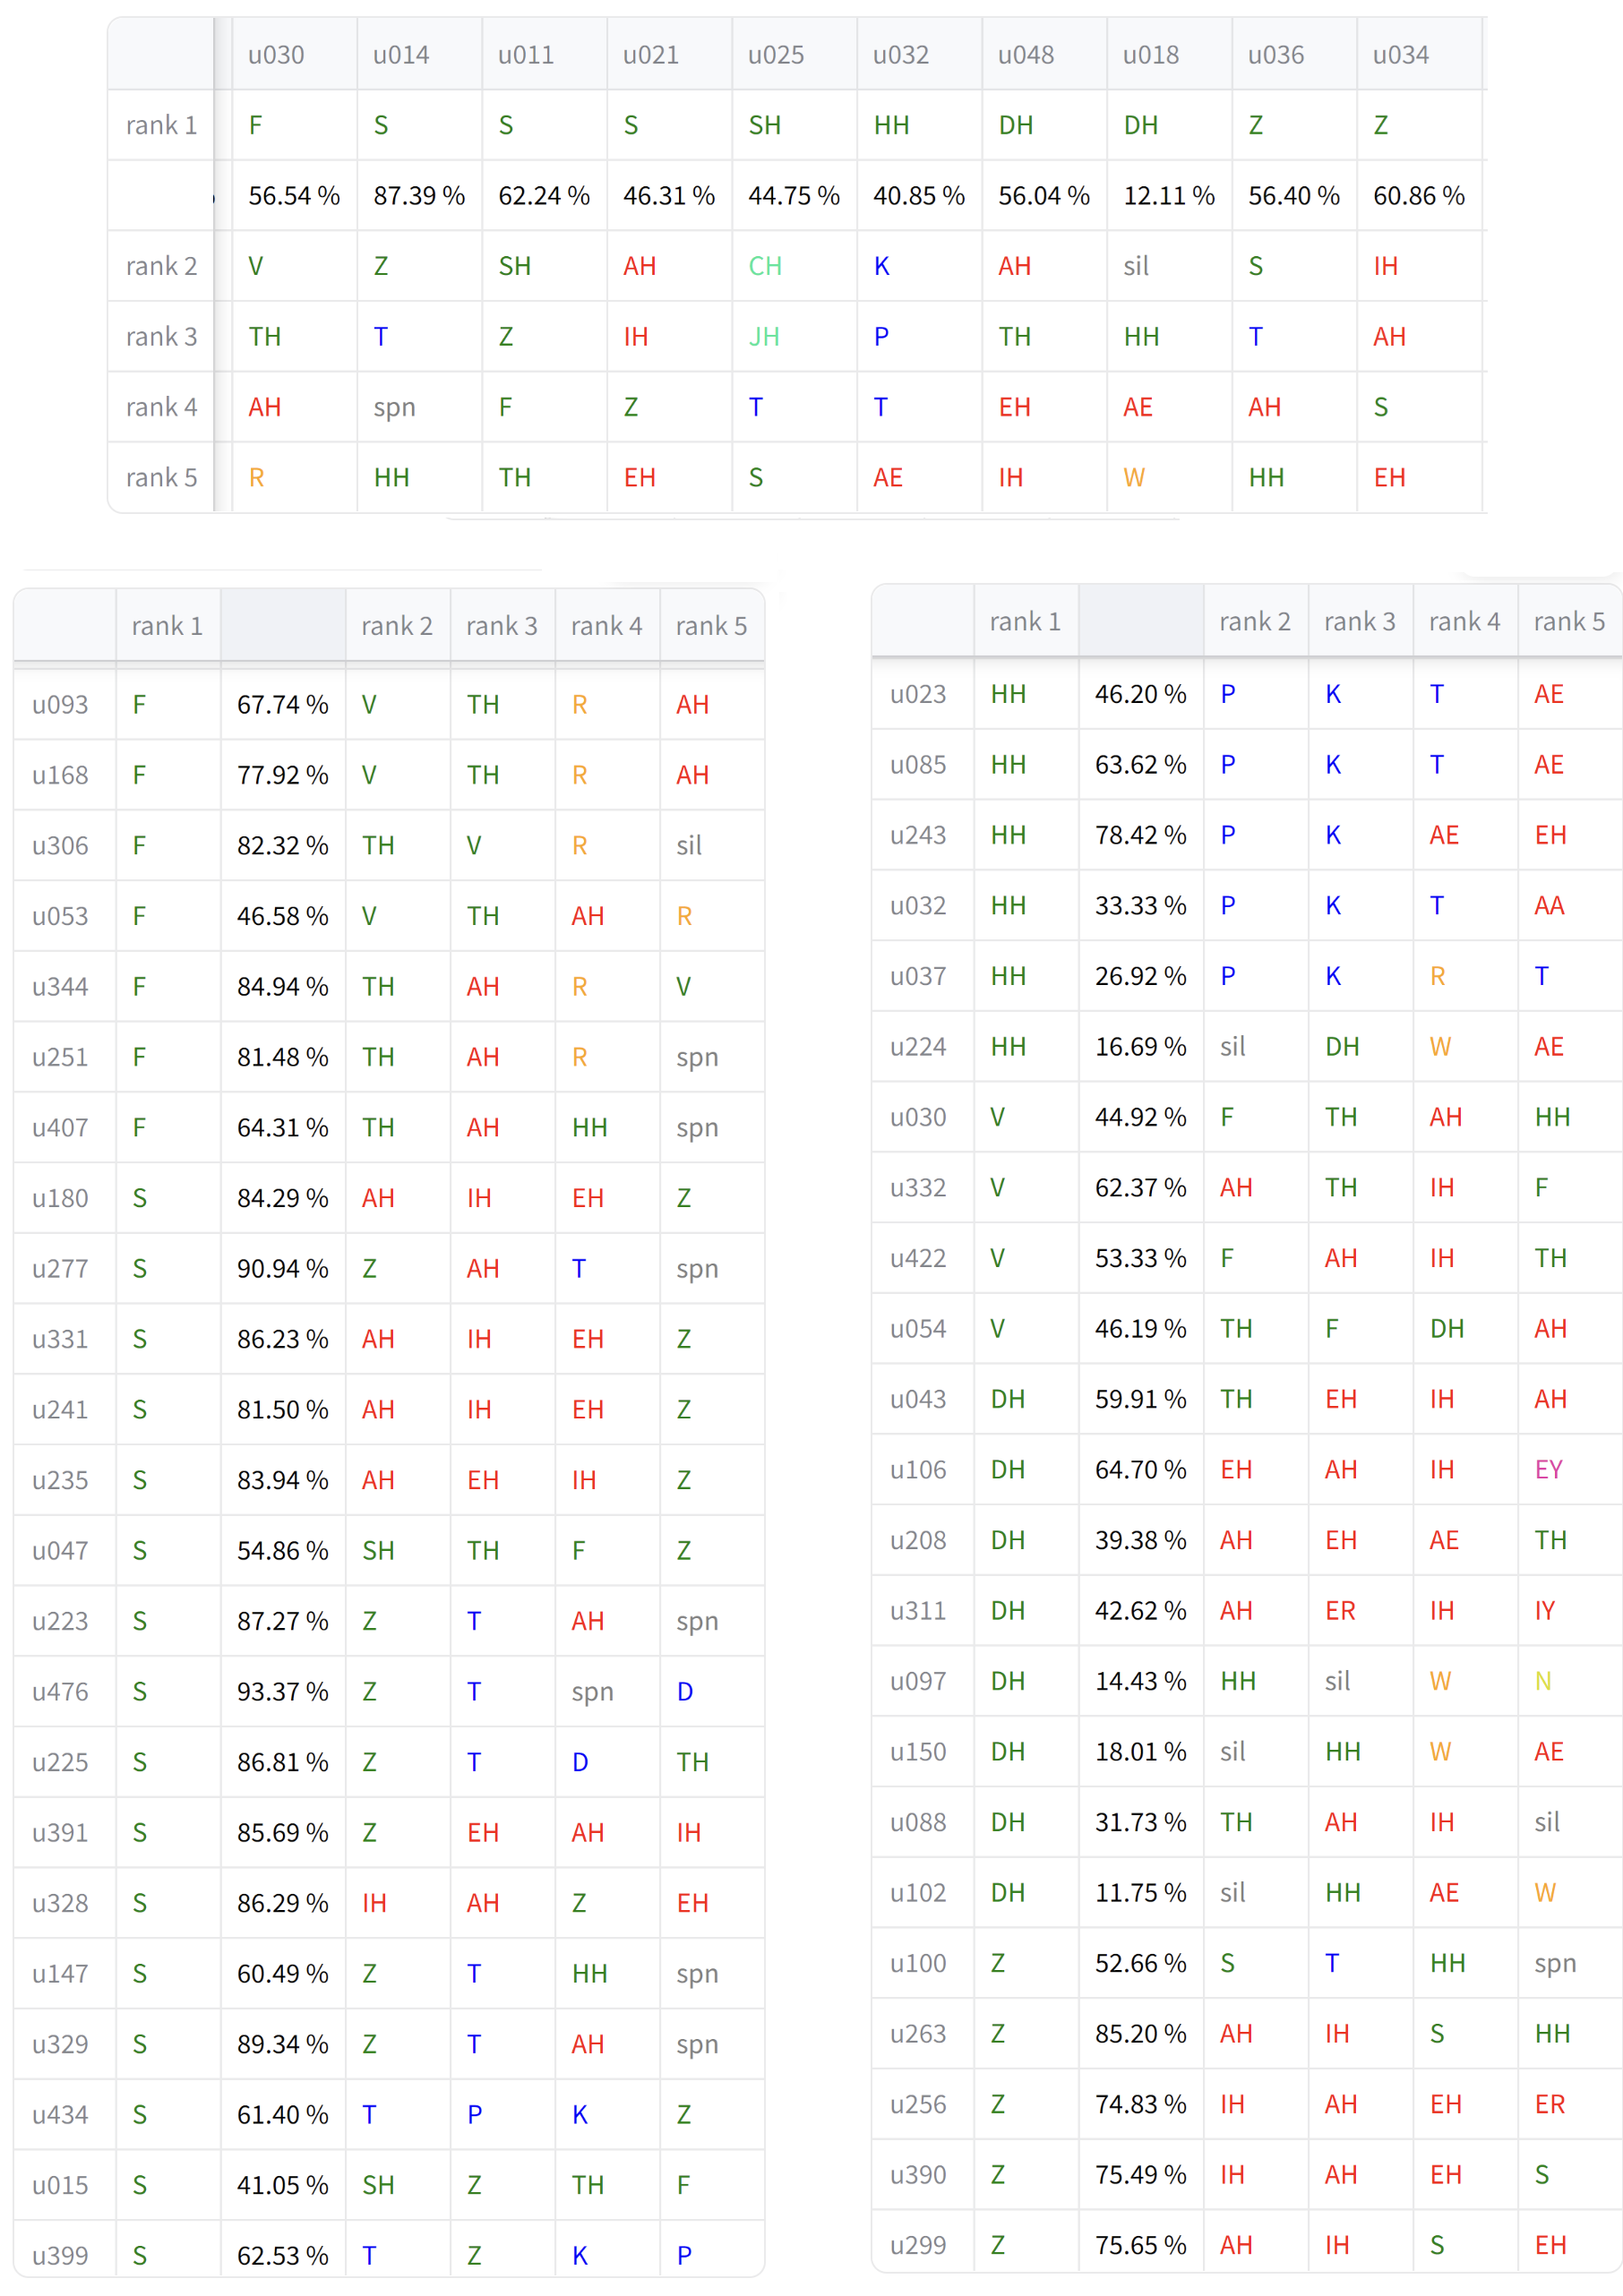
\includegraphics[width=\tempwidth]{chapters/fri_phn.png}
                 \caption{擦音}
                 \label{fig:hub-u050-ap0500-friobs}
             \end{subfigure}
             \vfill
             \begin{subfigure}{\textwidth}
                 \centering
                 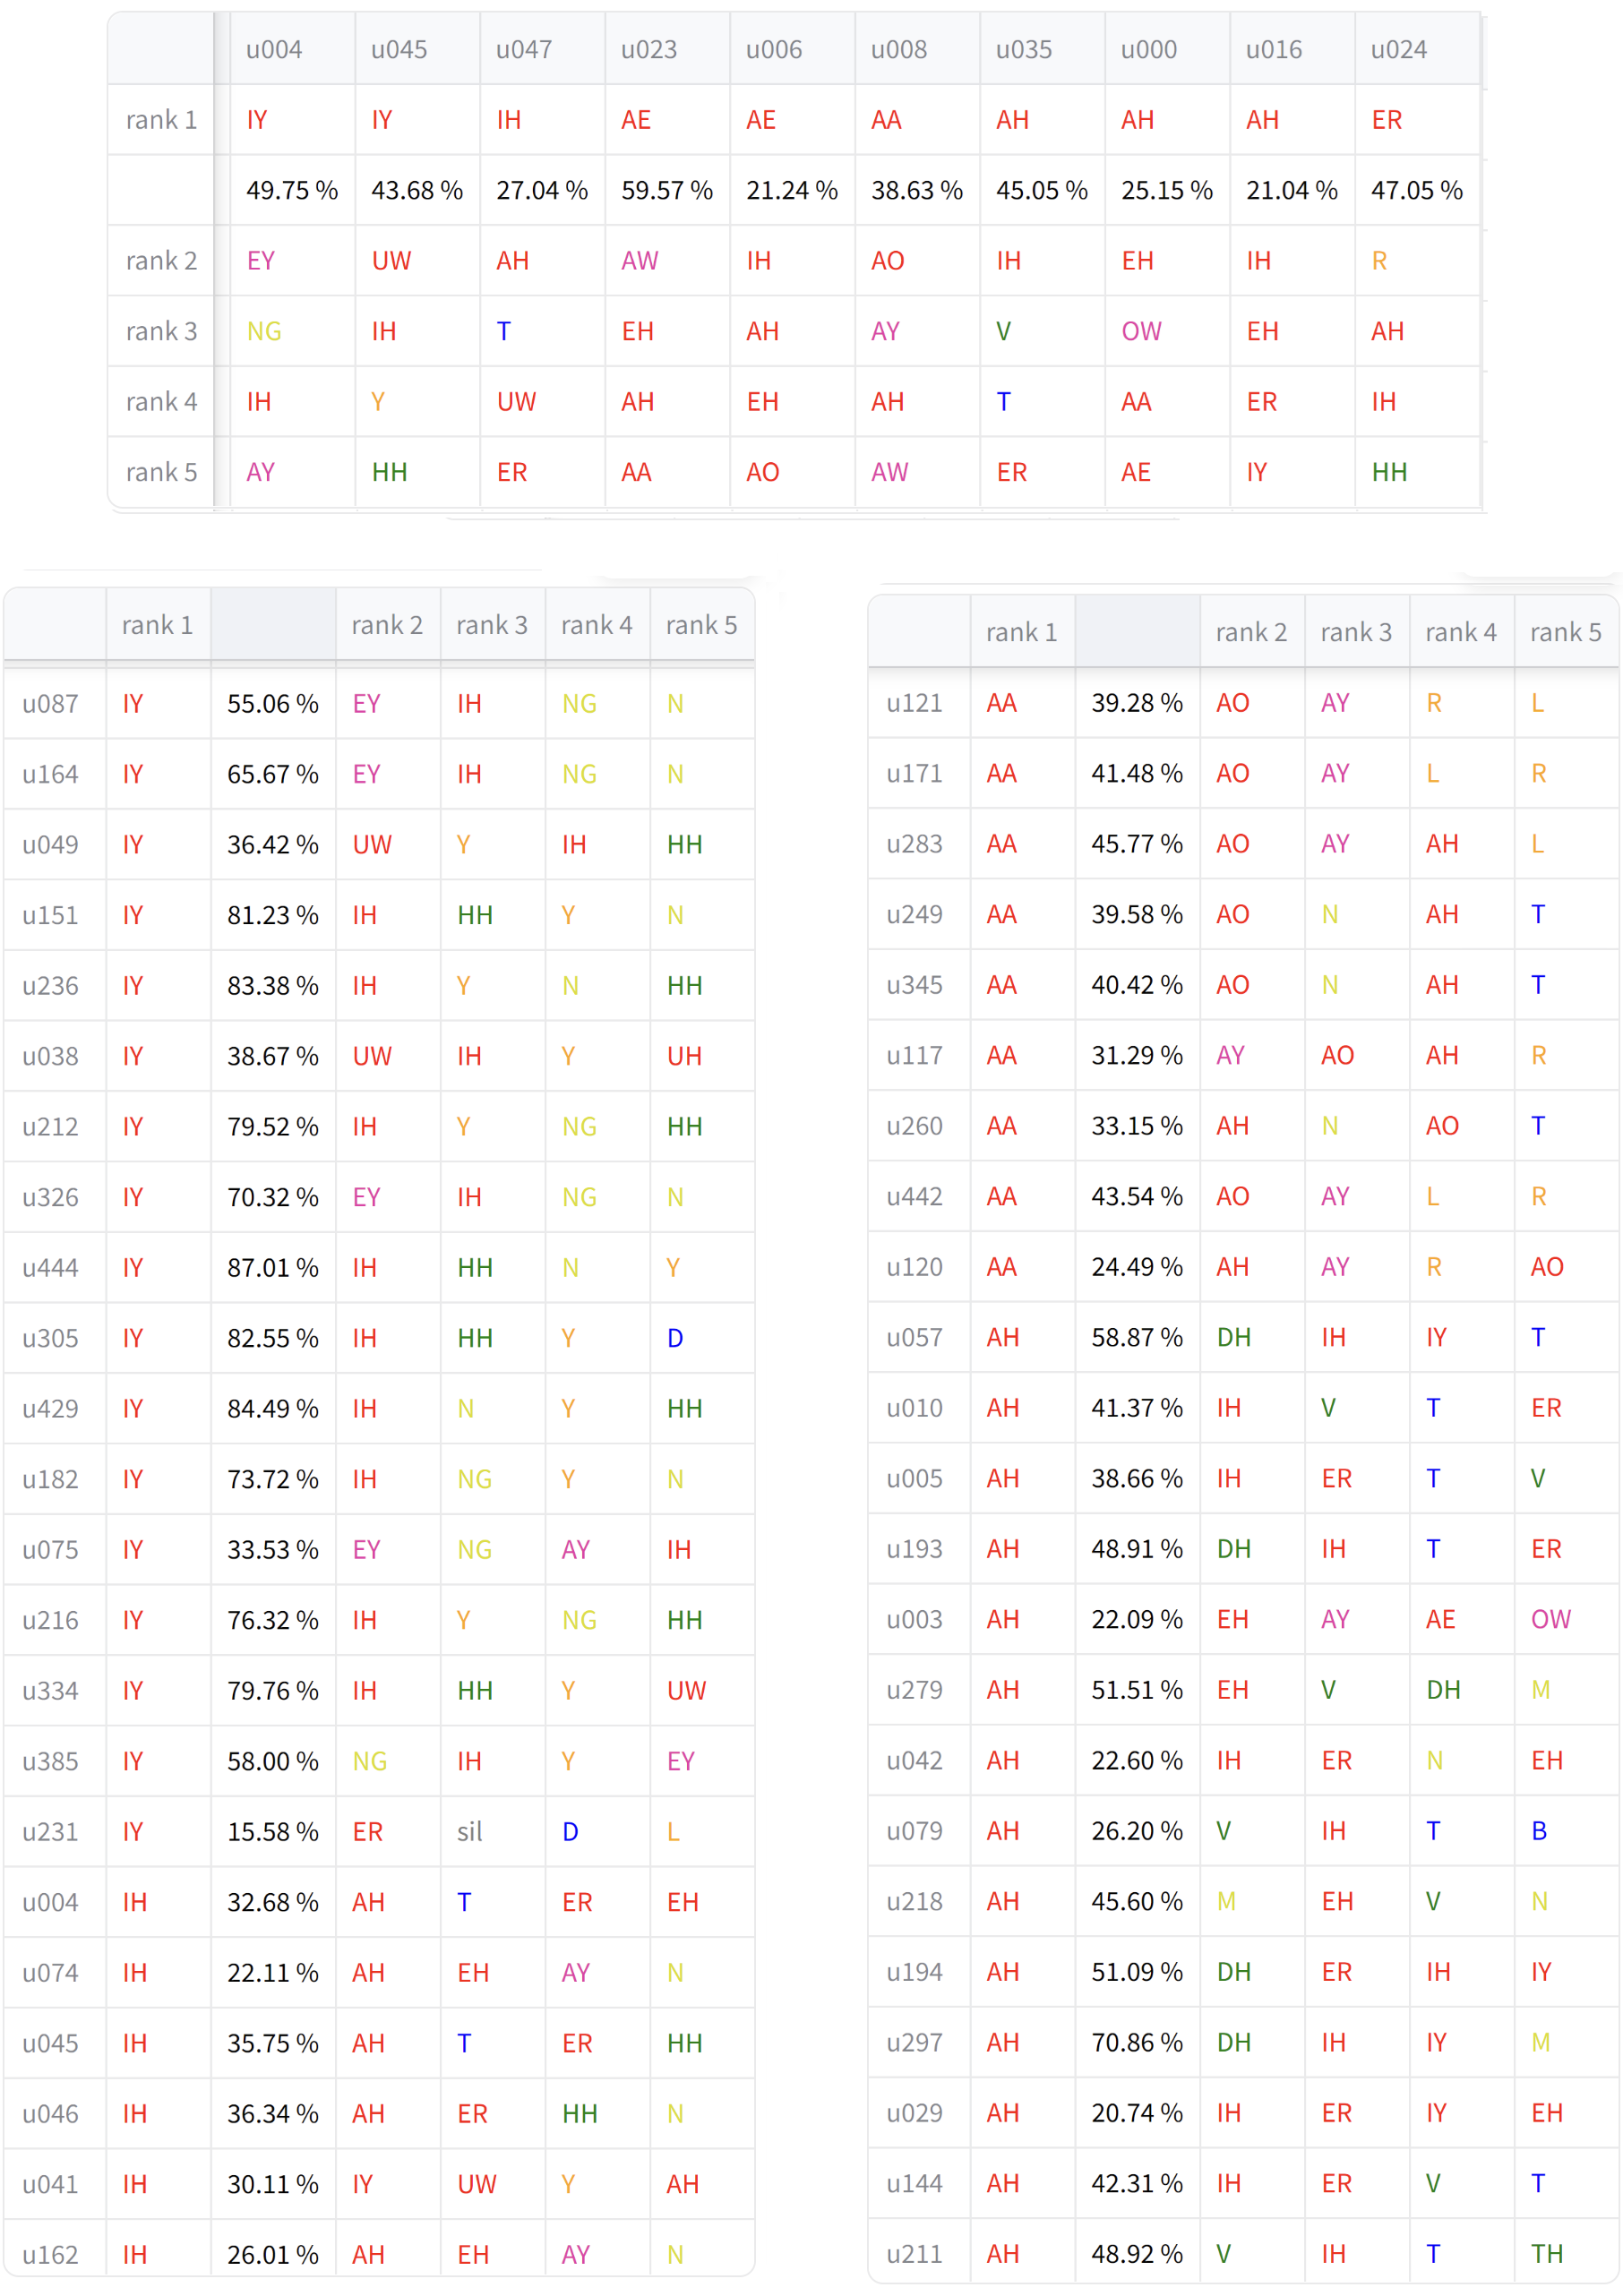
\includegraphics[width=\tempwidth]{chapters/vow_phn.png}
                 \caption{單元音}
                 \label{fig:hub-u050-ap0500-vowobs}
             \end{subfigure}

             \caption{HuBERT 表徵、K-平均演算法分群數 50,比較單一離散單元與使用 500 種次詞單位,}
             依據不同音位分類比較符記各自對應的前五高音位
             (上半部為離散單元,下半部為聲學片段。圖中的百分比為最高機率音位的條件機率 $p_{y|z}(i^*(j)|j)$)
                         \label{fig:hub-u050-phnobserver}
        \end{figure}
    }

\begin{figure}
    \centering
    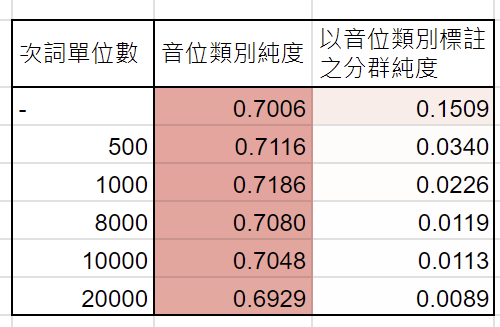
\includegraphics[width=0.5\linewidth]{.vscode/hub50clspur.png}
    \caption{Enter Caption}
    \label{fig:enter-label}
\end{figure}

\begin{figure}
    \centering
    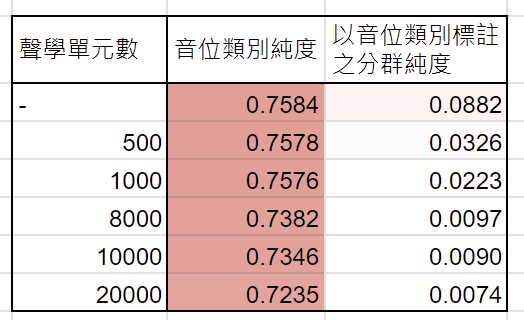
\includegraphics[width=0.5\linewidth]{hub100pcs--clupur.png}
    \caption{Enter Caption}
    \label{fig:enter-label}
\end{figure}
\subsubsection{各自離散單元視角的切入}
  接下來,我們也可以如同第三章對各自離散單元視角切入,觀察各個聲學片段對應音位之間的混淆關係,也就是對應機率前幾高音位之間是否依然如離散單元那樣存在特定特徵。圖 \ref{fig:hub-u050-phnobserver} 為 HuBERT 分群數 50 後取 500 個次詞單位所得聲學片段中,部分次詞單位所對應前五高機率音位對應排名,其中特別將塞音、擦音和單元音拿出來比較。圖中的上半部是離散單元,下半部則是聲學片段。從中可以發現,比起離散單元,由於聲學片段的符記數量更多,因此在維持對應音位之間相關性的同時,卻可以呈現出不同音位更細節的相關性。例如在圖 \ref{fig:hub-u050-ap0500-ploobs} 中,上半部顯示原先在離散單元時因為只有 50 個符記種類,因此只能看出 T、B 與 D 比較容易和哪些其他音位比較相關;但聲學片段卻可以呈現出 P、T、B、D 等更多細節的音位關係。
    (aff 圖)
    \begin{figure}
        \centering
        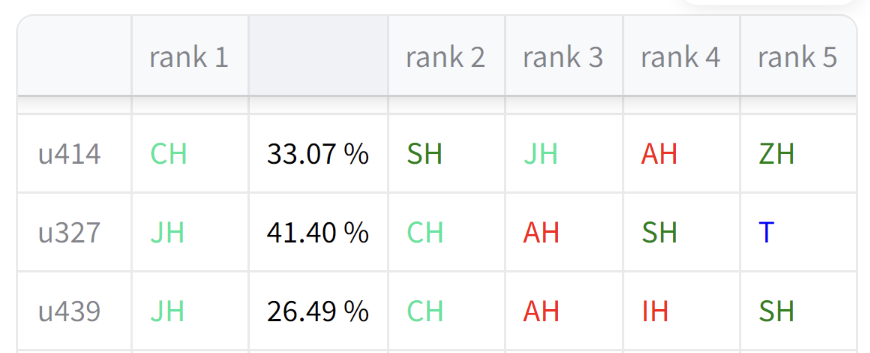
\includegraphics[width=0.5\linewidth]{chapters/aff-hub50-500.png}
        \caption{Enter Caption}
        \label{fig:aff}
    \end{figure}


        仿照第三章,我們也可以從「用音位分類為新標籤計算的純度」數據來證明這件事。隨著詞表大小的上升,整體的音位分類標註純度卻只有些微提升,而且愈來愈不明顯,幾乎沒什麼提升的空間了。 \par
        這很可能是因為分詞演算法本身的特性,聲學片段可以把帶有不同代表性音位的離散單元合在一起,因此整體對特定音位的代表性跟語音相關性就低上了不少。  \jcm{phn pur up, but pcls pur down}

\subsection{以音位角度切入}

\begin{figure}
    \centering
    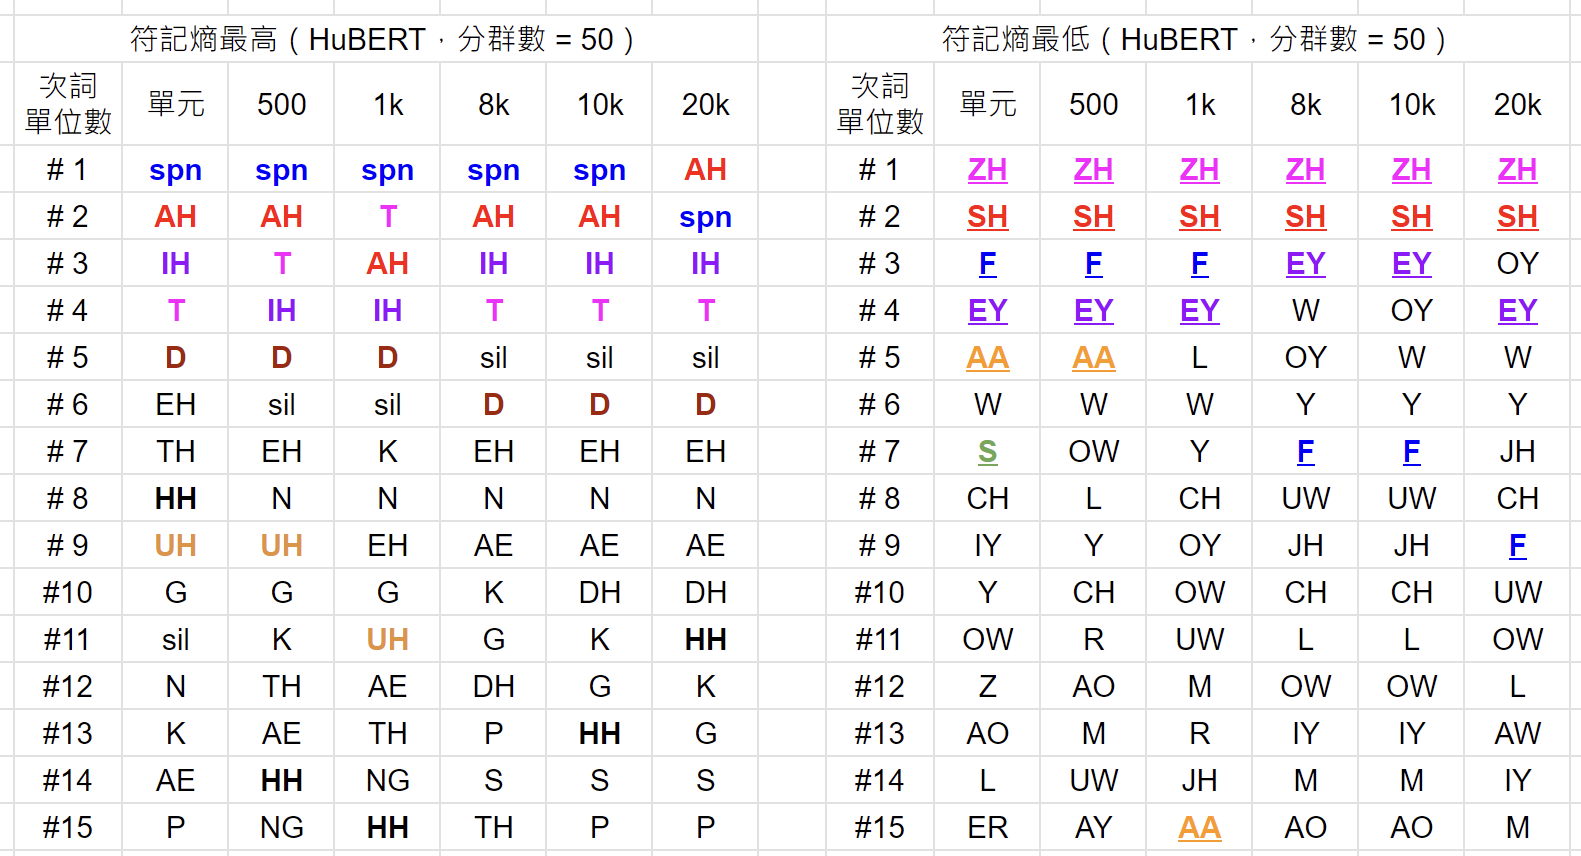
\includegraphics[width=0.5\linewidth]{phnrank-hub50pcs.png}
    \caption{Enter Caption}
    \label{fig:enter-label}
\end{figure}

\begin{figure}
    \centering
    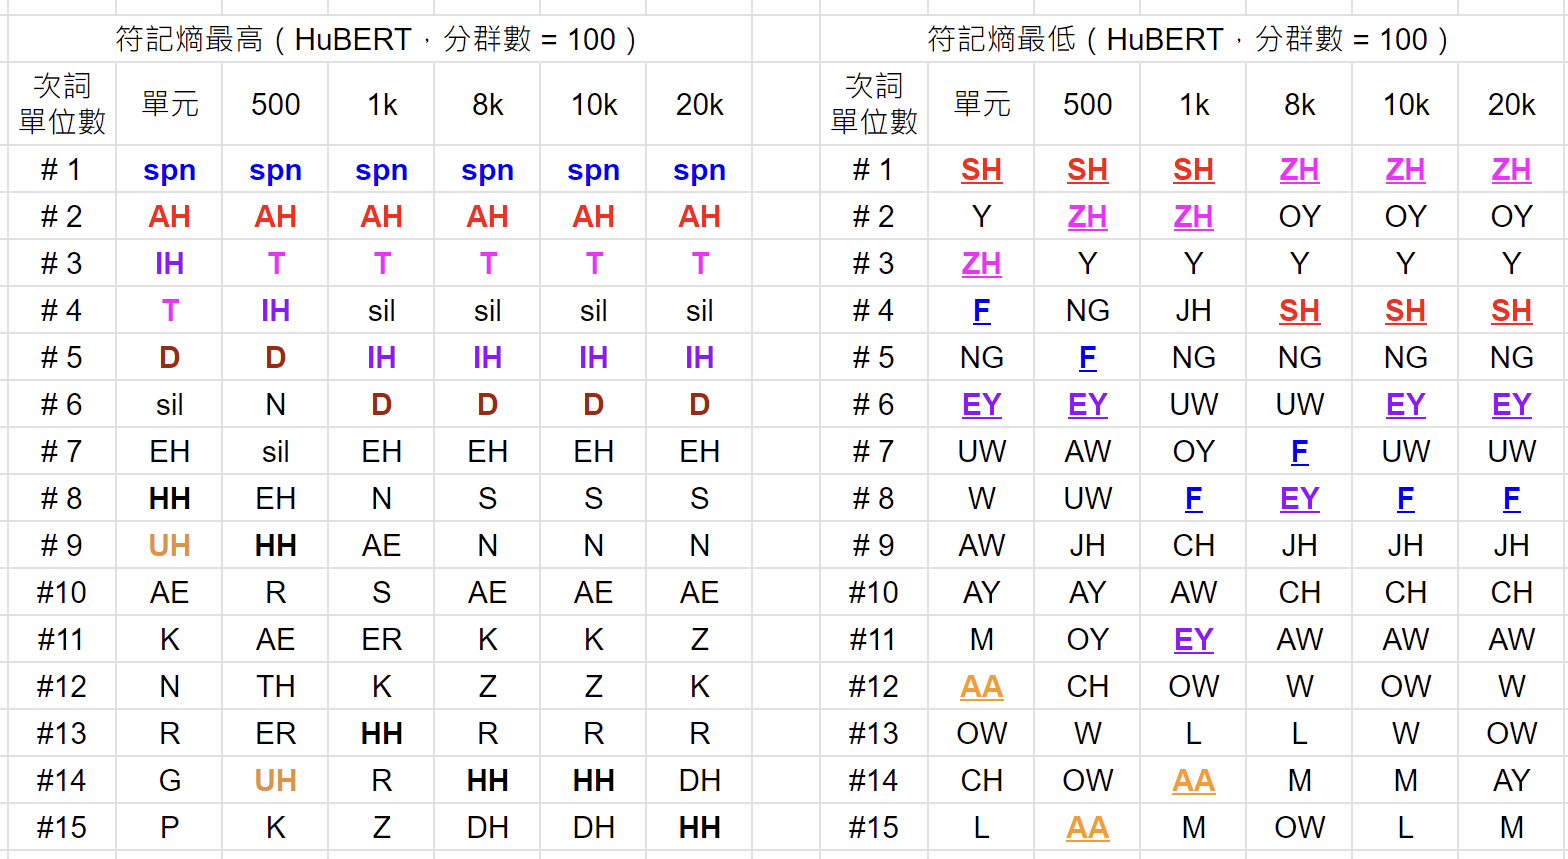
\includegraphics[width=0.5\linewidth]{phnrank-hub100pcs.png}
    \caption{Enter Caption}
    \label{fig:enter-label}
\end{figure}
  接著,我們轉而再度去以音位的角度切入,觀察各自音位的符記分佈集中程度。從圖 \ref{005} 中我們可以看到,整體排名趨勢幾乎與第三章不做分詞時的排名差不多,推論音位本身的容易或難以歸類的特性,單靠對語音表徵進行分群就已經可以不錯的發現這些現象。然而,即便分詞方法本身有機率將不同代表性音位的離散單元重新合在一起,卻也仍然大致維持了這個趨勢。因此,我們可以推論,音位本身對應符記的分散程度,不論是使用 K-平均演算法離散化,或是用分詞方法重新歸類次詞單位得到,這個分散程度的趨勢都是差不多的,音位本身的發音特徵或許是一個超出音框本身、影響範圍更廣泛的特性。 \par




{
\begin{figure}
    \centering
    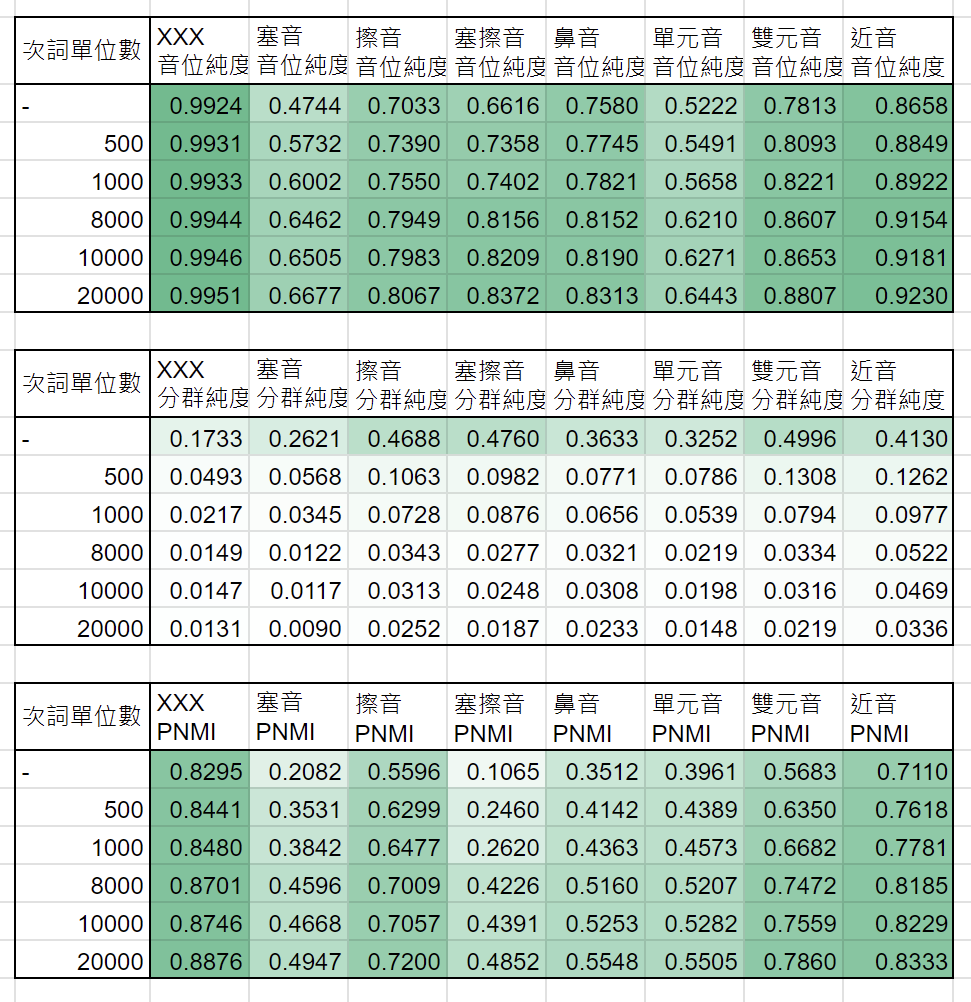
\includegraphics[width=0.5\linewidth]{hub50-ap-detailedpur.png}
    \caption{Enter Caption}
    \label{fig:hub50-ap-detailedpur}
\end{figure}
}


\begin{figure}
    \centering
    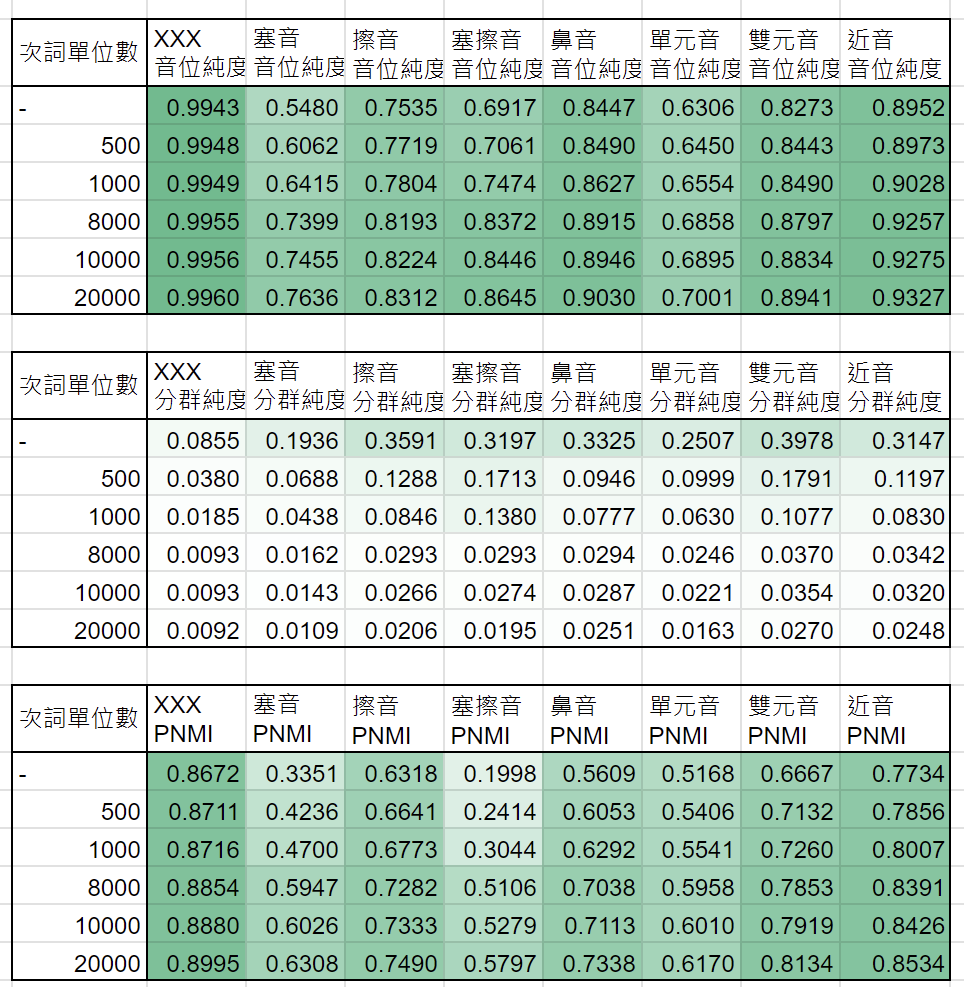
\includegraphics[width=0.5\linewidth]{hub100-ap-detailedpur.png}
    \caption{Enter Caption}
    \label{fig:hub100-ap-detailedpur}
\end{figure}


  
        最後,我們可以統計一下各音位分類的純度與相互資訊數據,與上一章節比對。由圖 \ref{fig:hub50-ap-detailedpur} 中可以看到,除了原本純度較低的塞音比較有所提升以外,其他純度較高的音位分類純度提升得很有限。儘管很不明顯,但整體大致仍然是有所提升的。


{
\begin{table}[!htbp]
    \centering
    \begin{subtable}[t]{\textwidth}
        \centering
        \begin{tabular}{|c|c|c|c|c|c|c|} \hline 
                詞表大小  & 音位純度 & 分群純度 & 音位熵 & 離散單元熵 &    PNMI & 長度壓縮比率 \\ \hline 
50 (未分詞)& 0.5256& 0.3382& 3.3152& 3.8681& 0.4993&1.0000\\ \hline 
                   500  &   0.5574   &  0.0829 &   3.3152  &  6.0282 & 0.5357 & 0.3486  \\ \hline %%  1.7758       
                  1000  &   0.5744   &  0.0556 &   3.3152  &  6.6594 & 0.5466 & 0.2992  \\ \hline %%  1.8120       
                  8000  &   0.5957   &  0.0257 &   3.3152  &  8.5192 & 0.5729 & 0.2074  \\ \hline %%  1.8993       
                 10000  &   0.5955   &  0.0238 &   3.3152  &  8.7207 & 0.5750 & 0.2007  \\ \hline %%  1.9063       
                 20000  &   0.5921   &  0.0182 &   3.3152  &  9.3527 & 0.5820 & 0.1819  \\ \hline %%  1.9293       
        \end{tabular}
\caption{群數 = 50}
        \label{tab:ch4-hubert-phn-clu050}
    \end{subtable}        
    \jefftablesep        
    \begin{subtable}[t]{\textwidth}
        \centering
        \begin{tabular}{|c|c|c|c|c|c|c|} \hline 
                詞表大小  & 音位純度 & 分群純度 & 音位熵 & 離散單元熵 &    PNMI & 長度壓縮比率 \\ \hline 
100 (未分詞)& 0.6097& 0.2553& 3.3152& 4.5704& 0.5786&1.0000\\ \hline 
                   500  &   0.6260   &  0.0972 &   3.3152  &  6.0655 & 0.5990 & 0.4432  \\ \hline %%  1.9858       
                  1000  &   0.6372   &  0.0631 &   3.3152  &  6.7181 & 0.6089 & 0.3666  \\ \hline %%  2.0186       
                  8000  &   0.6536   &  0.0237 &   3.3152  &  8.5954 & 0.6308 & 0.2444  \\ \hline %%  2.0912       
                 10000  &   0.6527   &  0.0219 &   3.3152  &  8.7938 & 0.6324 & 0.2357  \\ \hline %%  2.0965       
                 20000  &   0.6490   &  0.0173 &   3.3152  &  9.4123 & 0.6378 & 0.2123  \\ \hline %%  2.1145       
        \end{tabular}
\caption{群數 = 100}
        \label{tab:ch4-hubert-phn-clu100}
    \end{subtable}        


\caption{HuBERT 模型在不同詞表大小時的音位分析數據}
    \label{tab:hubert-phn-results}
\end{table}

}  % tables
{

\begin{figure}
    \centering
    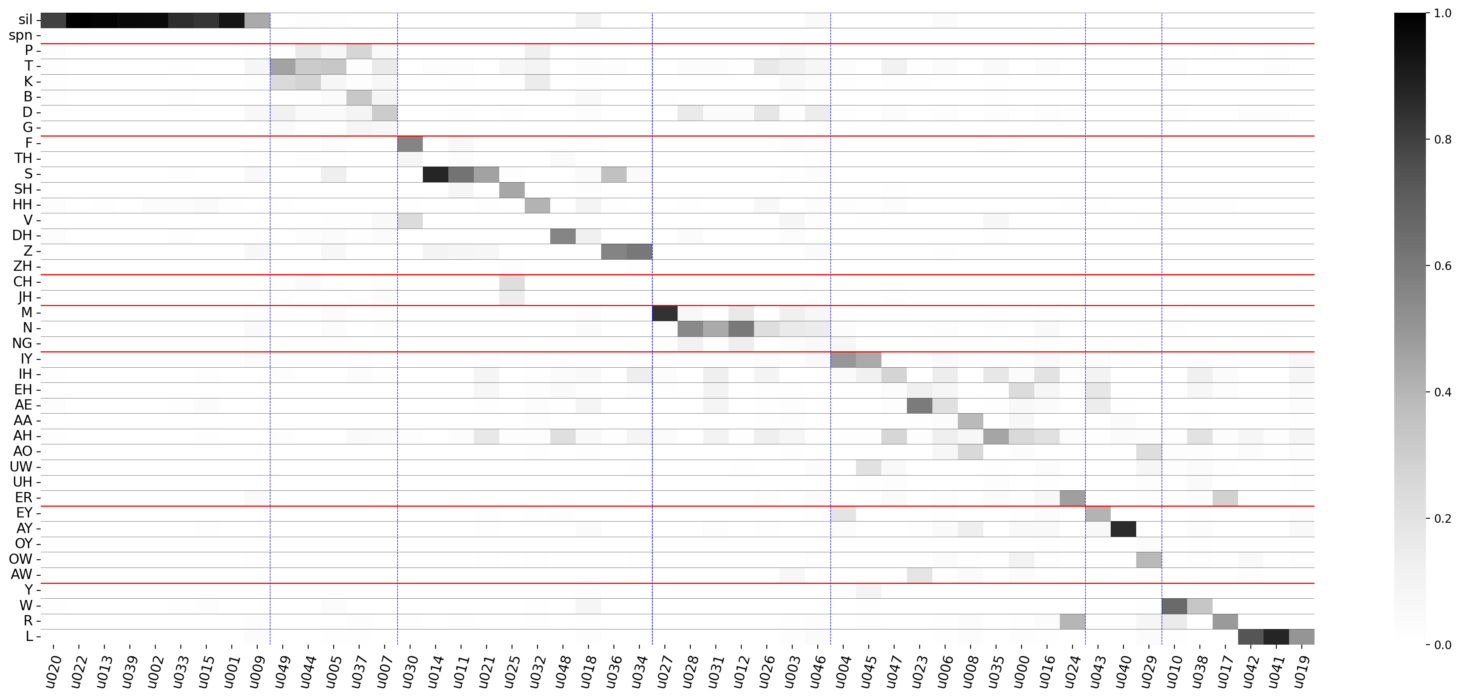
\includegraphics[width=1\linewidth]{feasiblefigs/ch4figs/hub-u050-ap0000-givenunit-byphn.png}
    \caption{hub-u050-ap0000-givenunit-byphn}
    \label{fig:hub-u050-ap0000-givenunit-byphn--detailed}
\end{figure}

\begin{figure}
    \centering
    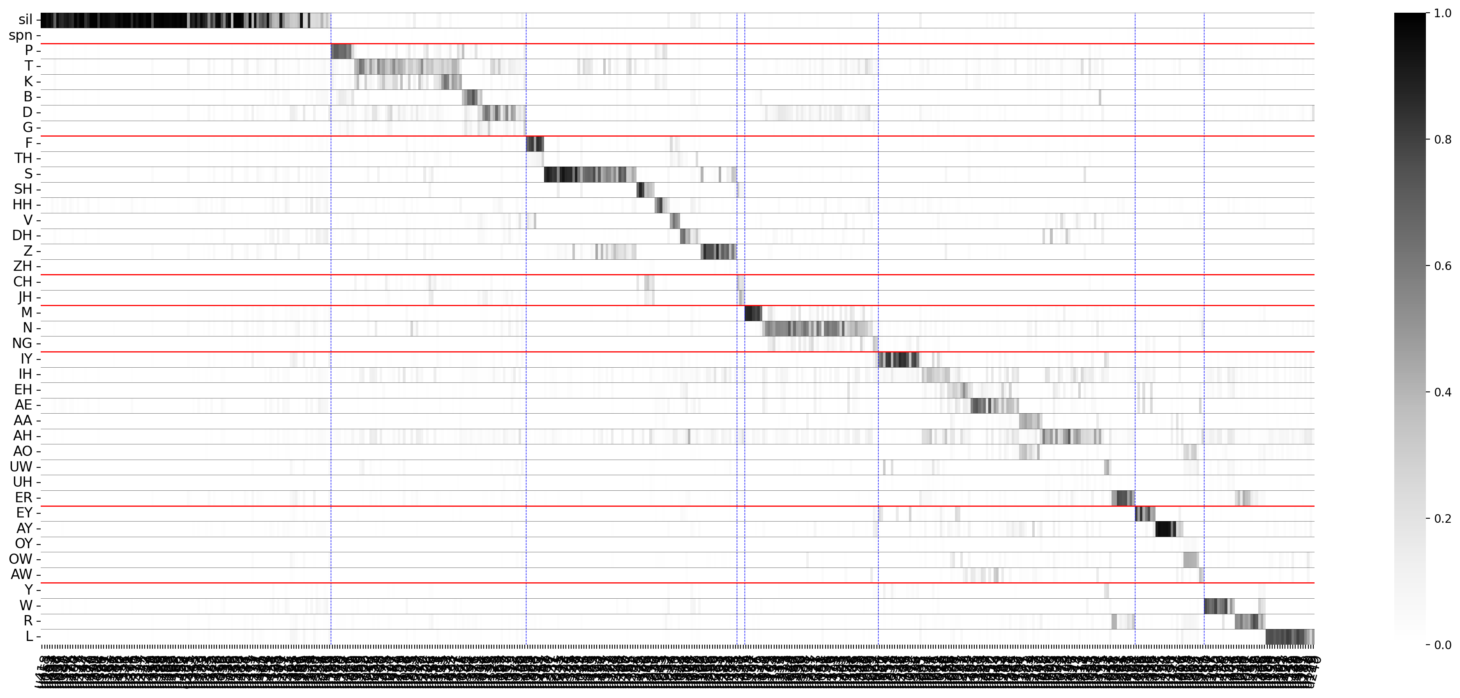
\includegraphics[width=1\linewidth]{feasiblefigs/ch4figs/hub-u050-ap0500-givenunit-byphn.png}
    \caption{hub-u050-ap0500-givenunit-byphn}
    \label{fig:hub-u050-ap0500-givenunit-byphn--detailed}
\end{figure}

\begin{figure}
    \centering
    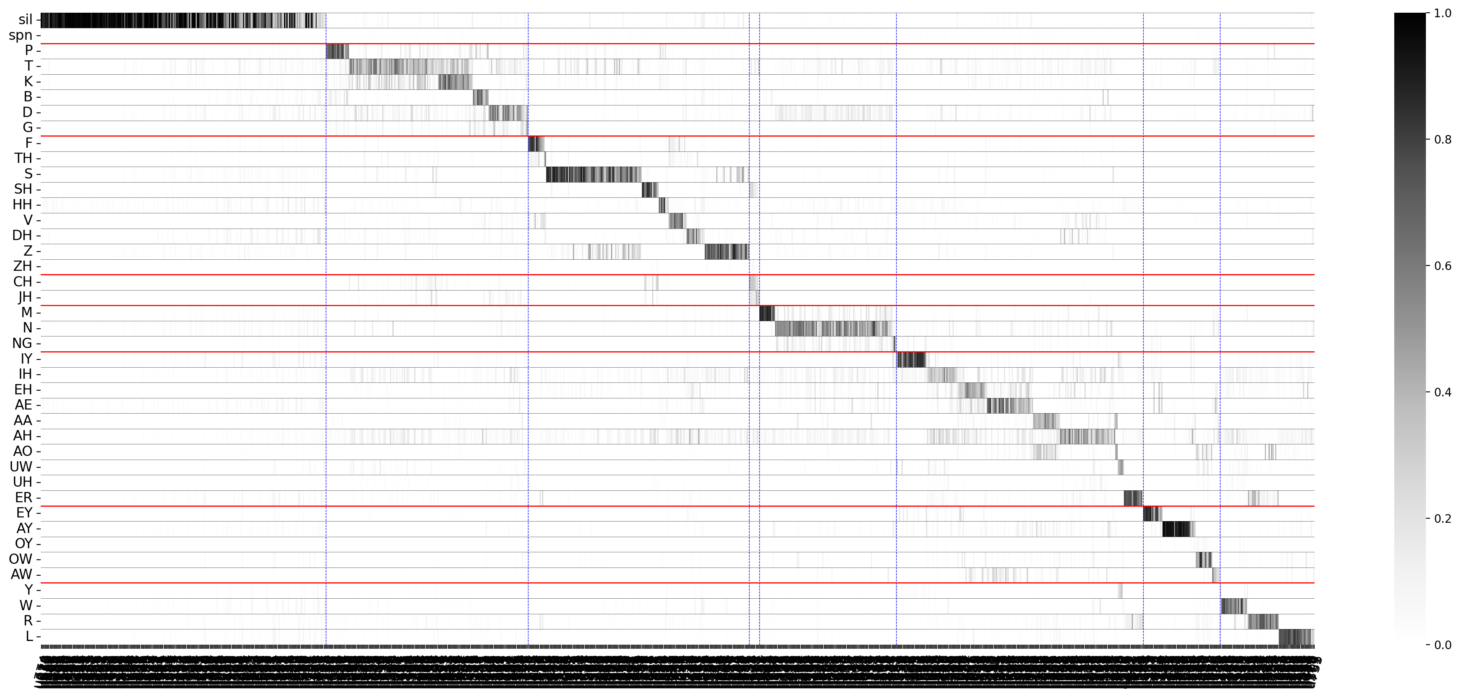
\includegraphics[width=1\linewidth]{feasiblefigs/ch4figs/hub-u050-ap1000-givenunit-byphn.png}
    \caption{hub-u050-ap1000-givenunit-byphn}
    \label{fig:hub-u050-ap1000-givenunit-byphn--detailed}
\end{figure}

\begin{figure}
    \centering
    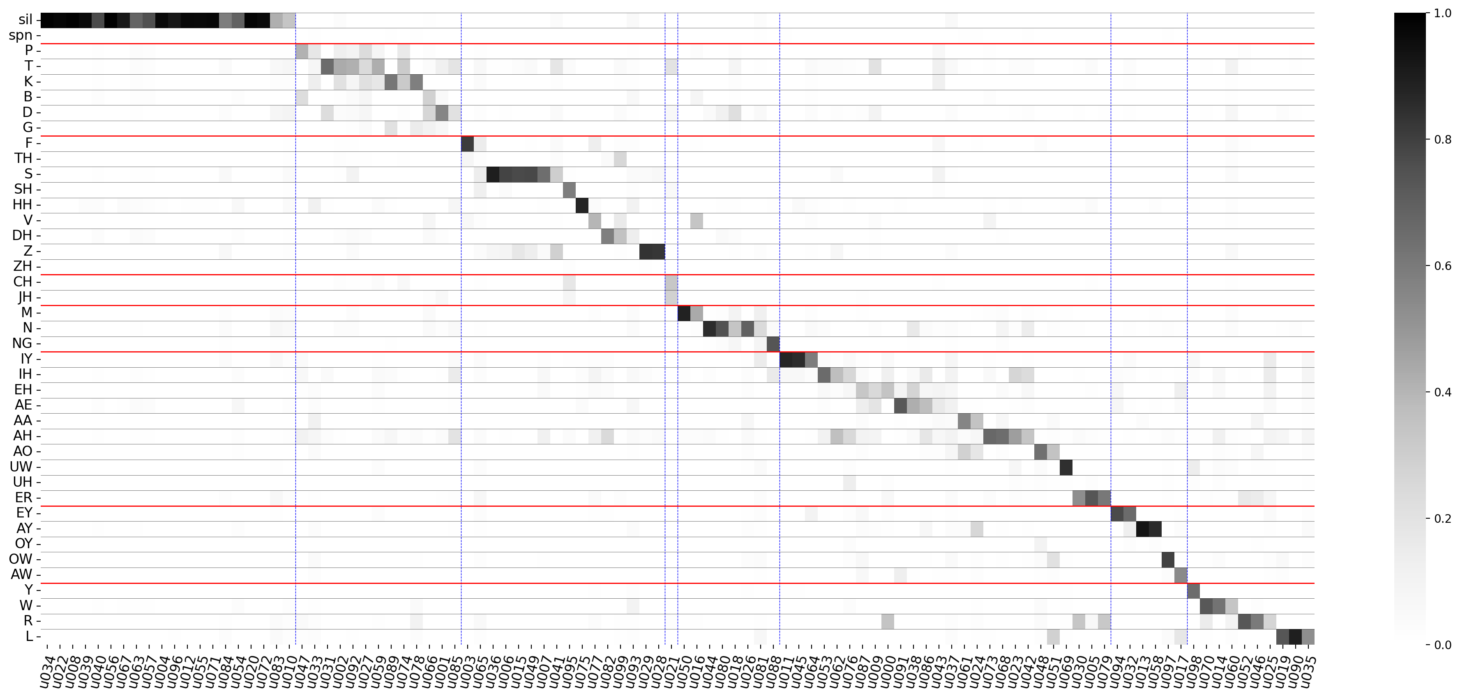
\includegraphics[width=1\linewidth]{feasiblefigs/ch4figs/hub-u100-ap0000-givenunit-byphn.png}
    \caption{hub-u100-ap0000-givenunit-byphn}
    \label{fig:hub-u100-ap0000-givenunit-byphn--detailed}
\end{figure}
\begin{figure}
    \centering
    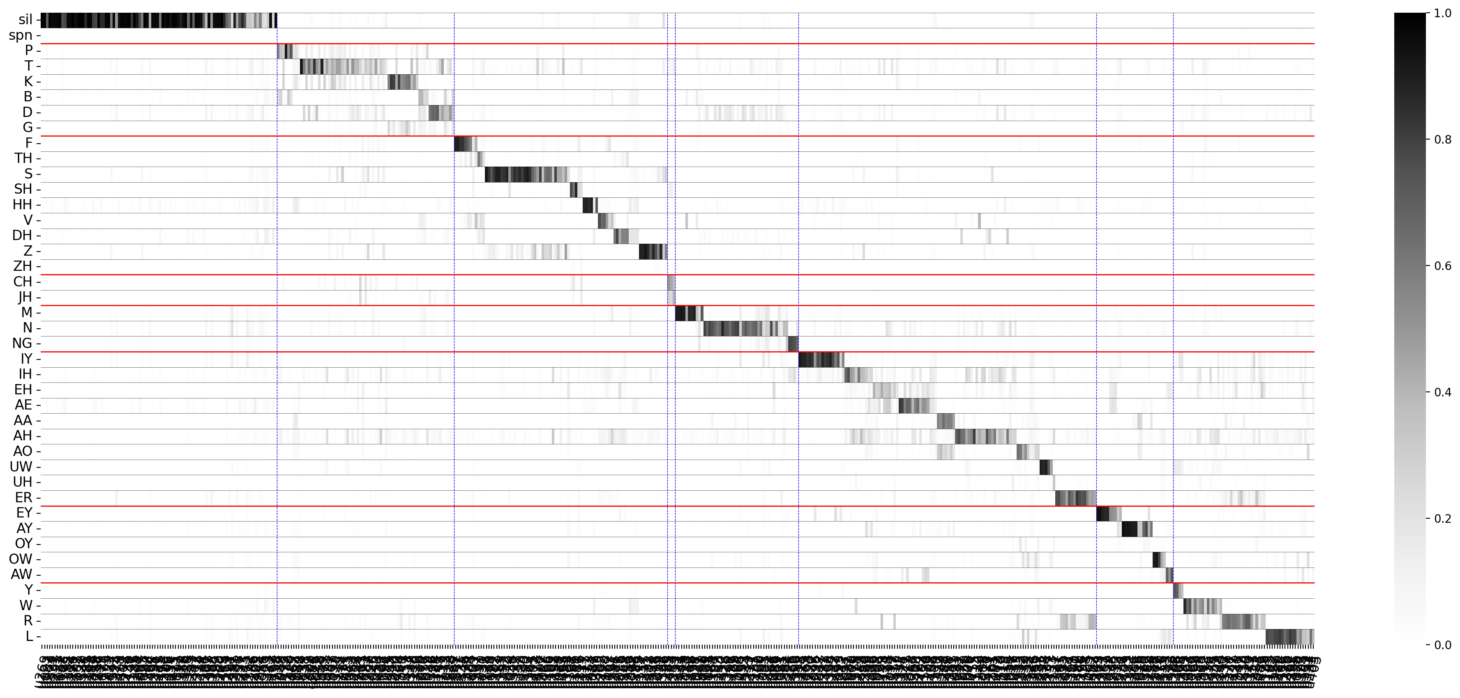
\includegraphics[width=1\linewidth]{feasiblefigs/ch4figs/hub-u100-ap0500-givenunit-byphn.png}
    \caption{hub-u100-ap0500-givenunit-byphn}
    \label{fig:hub-u100-ap0500-givenunit-byphn--detailed}
\end{figure}
\begin{figure}
    \centering
    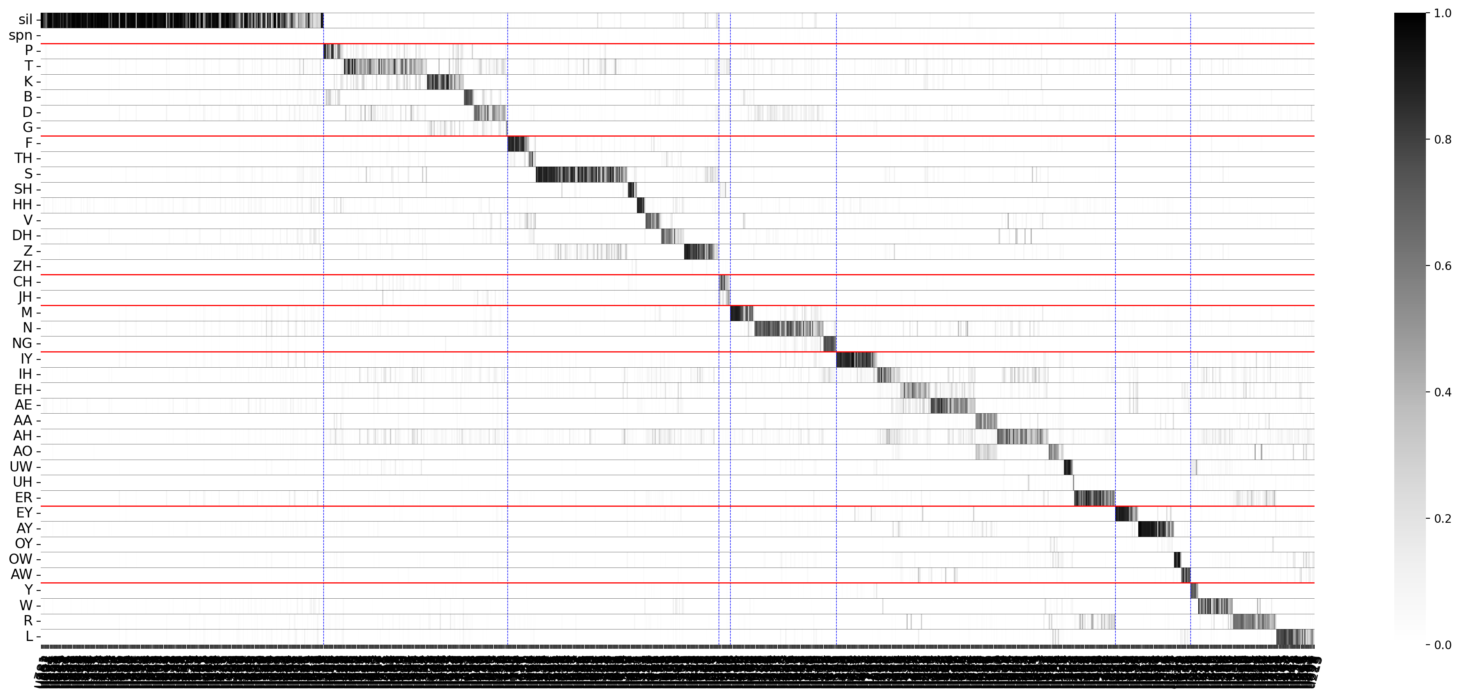
\includegraphics[width=1\linewidth]{feasiblefigs/ch4figs/hub-u100-ap1000-givenunit-byphn.png}
    \caption{hub-u100-ap1000-givenunit-byphn}
    \label{fig:hub-u100-ap1000-givenunit-byphn--detailed}
\end{figure}
}  % heatmaps


\jcm{section{分析結果} }
\jcm{  以下數據中的「長度壓縮比率」係指透過分詞方法後,每一個句子的「單詞」數與原先離散單元的數量相比之比值。由於長度壓縮比率是針對離散單元分詞所得到,與標註無關,因此只在音位分析的表格上呈現。}
\jcm{subsection{基於各自音位的分析}}
\jcm{  首先,為了比較不同詞表大小對於純度、相互資訊等數據的影響,先分別固定語音模型為 HuBERT 和 Wav2vec 2.0,在離散單元的分群數量為 50、100、200 三種設定下,觀察詞表大小造成的變化。由 HuBERT (表 \ref{tab:hubert-phn-results})和 Wav2vec 2.0(表 \ref{tab:w2v2-phn-results})的數據比較可觀察到,詞表大小上升除了使得音位純度提高以外,相互資訊也是隨之提高的,可以發現使用分詞方法並給予足夠大的詞表,對於找出語音中的資訊確實有所幫助。}
\jcm{        接著從另一個角度切入,比較同樣都是離散單元分群數為 200 的條件下,不同語音基石模型的分析數據。由表 \ref{tab:ch4-models-phn} 可以發現,HuBERT 模型在音位純度與相互資訊勝過其他模型,這個結論與上一章節是一致的。}
\jcm{        有趣的是,觀察長度壓縮比率可以發現,CPC 模型在分詞演算法的引入後,能夠使序列變得最短,但同時在音位純度與相互資訊上也有所犧牲;而 HuBERT 雖然在這些分析數據上高過其他三者,卻同時達成了比 Wav2vec 2.0 和 LogMel 更好的壓縮比率。因此綜合看來,這很可能是目前使用語音離散單元進行研究時,HuBERT 模型仍然是領域內首選的緣由。}
\jcm{                
\begin{table}[!htbp]
    \centering
    \begin{subtable}[t]{\textwidth}
        \centering
        \begin{tabular}{|c|c|c|c|c|c|c|} \hline 
                詞表大小  & 音位純度 & 分群純度 & 音位熵 & 離散單元熵 &    PNMI & 長度壓縮比率 \\ \hline 
50 (未分詞)& 0.5256& 0.3382& 3.3152& 3.8681& 0.4993&1.0000\\ \hline 
                   500  &   0.5574   &  0.0829 &   3.3152  &  6.0282 & 0.5357 & 0.3486  \\ \hline %%  1.7758       
                  1000  &   0.5744   &  0.0556 &   3.3152  &  6.6594 & 0.5466 & 0.2992  \\ \hline %%  1.8120       
                  8000  &   0.5957   &  0.0257 &   3.3152  &  8.5192 & 0.5729 & 0.2074  \\ \hline %%  1.8993       
                 10000  &   0.5955   &  0.0238 &   3.3152  &  8.7207 & 0.5750 & 0.2007  \\ \hline %%  1.9063       
                 20000  &   0.5921   &  0.0182 &   3.3152  &  9.3527 & 0.5820 & 0.1819  \\ \hline %%  1.9293       
        \end{tabular}
\caption{群數 = 50}
        \label{tab:ch4-hubert-phn-clu050}
    \end{subtable}        

    \jefftablesep        

    \begin{subtable}[t]{\textwidth}
        \centering
        \begin{tabular}{|c|c|c|c|c|c|c|} \hline 
                詞表大小  & 音位純度 & 分群純度 & 音位熵 & 離散單元熵 &    PNMI & 長度壓縮比率 \\ \hline 
100 (未分詞)& 0.6097& 0.2553& 3.3152& 4.5704& 0.5786&1.0000\\ \hline 
                   500  &   0.6260   &  0.0972 &   3.3152  &  6.0655 & 0.5990 & 0.4432  \\ \hline %%  1.9858       
                  1000  &   0.6372   &  0.0631 &   3.3152  &  6.7181 & 0.6089 & 0.3666  \\ \hline %%  2.0186       
                  8000  &   0.6536   &  0.0237 &   3.3152  &  8.5954 & 0.6308 & 0.2444  \\ \hline %%  2.0912       
                 10000  &   0.6527   &  0.0219 &   3.3152  &  8.7938 & 0.6324 & 0.2357  \\ \hline %%  2.0965       
                 20000  &   0.6490   &  0.0173 &   3.3152  &  9.4123 & 0.6378 & 0.2123  \\ \hline %%  2.1145       
        \end{tabular}
\caption{群數 = 100}
        \label{tab:ch4-hubert-phn-clu100}
    \end{subtable}        

    \jefftablesep        

    \begin{subtable}[t]{\textwidth}
        \centering
        \begin{tabular}{|c|c|c|c|c|c|c|} \hline 
                詞表大小  & 音位純度 & 分群純度 & 音位熵 & 離散單元熵 &    PNMI & 長度壓縮比率 \\ \hline 
200 (未分詞)& 0.6474& 0.1644& 3.3152& 5.2681& 0.6289&1.0000\\ \hline 
                   500  &   0.6471   &  0.0930 &   3.3152  &  6.0986 & 0.6314 & 0.5995  \\ \hline %%  2.0934       
                  1000  &   0.6540   &  0.0558 &   3.3152  &  6.7786 & 0.6382 & 0.4609  \\ \hline %%  2.1156       
                  8000  &   0.6690   &  0.0208 &   3.3152  &  8.6544 & 0.6567 & 0.2874  \\ \hline %%  2.1769       
                 10000  &   0.6693   &  0.0189 &   3.3152  &  8.8535 & 0.6584 & 0.2764  \\ \hline %%  2.1826       
                 20000  &   0.6684   &  0.0144 &   3.3152  &  9.4737 & 0.6636 & 0.2467  \\ \hline %%  2.1999      
        \end{tabular}
\caption{群數 = 200}
        \label{tab:ch4-hubert-phn-clu200}
    \end{subtable}        

\caption{HuBERT 模型在不同詞表大小時的音位分析數據}
    \label{tab:hubert-phn-results}
\end{table}



\begin{table}[!htbp]
    \centering
    \begin{subtable}[t]{\textwidth}
        \centering
        \begin{tabular}{|c|c|c|c|c|c|c|} \hline 
                詞表大小  & 音位純度 & 分群純度 & 音位熵 & 離散單元熵 &    PNMI & 長度壓縮比率 \\ \hline 
 50 (未分詞)&  0.4006 &   0.2676 & 3.3152 &     3.8215 & 0.3706&1.0000\\ \hline 
                  500  &   0.4295&     0.0594    &3.3152 &   6.0328  &       0.4027 &0.3943 \\ \hline %%  
                 1000  &   0.4411&     0.0456    &3.3152 &   6.6250  &       0.4132 &0.3448 \\ \hline %%  
                 8000  &   0.4676&     0.0239    &3.3152 &   8.4954  &       0.4438 &0.2429 \\ \hline %%  
                10000  &   0.4705&     0.0227    &3.3152 &   8.6966  &       0.4477 &0.2352 \\ \hline %%  
                20000  &   0.4753&     0.0185    &3.3152 &   9.3471  &       0.4587 &0.2132 \\ \hline %%  
        \end{tabular}
\caption{群數 = 50}
        \label{tab:ch4-w2v2-phn-clu050}
    \end{subtable}        

    \jefftablesep        

    \begin{subtable}[t]{\textwidth}
        \centering
        \begin{tabular}{|c|c|c|c|c|c|c|} \hline 
                詞表大小  & 音位純度 & 分群純度 & 音位熵 & 離散單元熵 &    PNMI & 長度壓縮比率 \\ \hline 
 100 (未分詞)&0.4877 &   0.2118 & 3.3152 &     4.5284 & 0.4596&1.0000\\ \hline 
                  500  &   0.5016&     0.0697    &3.3152 &   6.0769  &       0.4784 &0.4926 \\ \hline %%  
                 1000  &   0.5108&     0.0444    &3.3152 &   6.7265  &       0.4867 &0.4160 \\ \hline %%  
                 8000  &   0.5427&     0.0215    &3.3152 &   8.5576  &       0.5180 &0.2895 \\ \hline %%  
                10000  &   0.5451&     0.0203    &3.3152 &   8.7602  &       0.5218 &0.2797 \\ \hline %%  
                20000  &   0.5531&     0.0162    &3.3152 &   9.4070  &       0.5345 &0.2526 \\ \hline %%  
        \end{tabular}
\caption{群數 = 100}
        \label{tab:ch4-w2v2-phn-clu100}
    \end{subtable}        

    \jefftablesep        

    \begin{subtable}[t]{\textwidth}
        \centering
        \begin{tabular}{|c|c|c|c|c|c|c|} \hline 
                詞表大小  & 音位純度 & 分群純度 & 音位熵 & 離散單元熵 &    PNMI & 長度壓縮比率 \\ \hline 
 200 (未分詞)&  0.5427 &   0.1467 & 3.3152 &     5.2173 & 0.5188 &1.0000\\ \hline 
                  500  &   0.5481&     0.0846    &3.3152 &   6.0756  &       0.5276 &0.6418 \\ \hline %%  
                 1000  &   0.5549&     0.0509    &3.3152 &   6.7483  &       0.5347 &0.5178 \\ \hline %%  
                 8000  &   0.5803&     0.0180    &3.3152 &   8.6065  &       0.5632 &0.3498 \\ \hline %%  
                10000  &   0.5828&     0.0166    &3.3152 &   8.8136  &       0.5668 &0.3373 \\ \hline %%  
                20000  &   0.5917&     0.0129    &3.3152 &   9.4561  &       0.5794 &0.3026  \\ \hline %%  
        \end{tabular}
\caption{群數 = 200}
        \label{tab:ch4-w2v2-phn-clu200}
    \end{subtable}        

\caption{Wav2vec 2.0 模型在不同詞表大小時的音位分析數據}
    \label{tab:w2v2-phn-results}
\end{table}




\begin{table}[!htbp]
    \centering
    \begin{subtable}[t]{\textwidth}
        \centering
        \begin{tabular}{|c|c|c|c|c|c|c|} \hline 
                詞表大小  & 音位純度 & 分群純度 & 音位熵 & 離散單元熵 &    PNMI & 長度壓縮比率 \\ \hline 
200 (未分詞)&   0.6474 &   0.1644 & 3.3152 &     5.2681 & 0.6289 &1.0000\\ \hline 
                    500   & 0.6471   & 0.0930   & 3.3152 &  6.0986    &  0.6314 &  0.5995  \\ \hline %%   2.0934
                   1000   & 0.6540   & 0.0558   & 3.3152 &  6.7786    &  0.6382 &  0.4609  \\ \hline %%   2.1156
                  10000   & 0.6693   & 0.0189   & 3.3152 &  8.8535    &  0.6584 &  0.2764  \\ \hline %%   2.1826
        \end{tabular}
\caption{HuBERT}
        \label{tab:ch4-phn-model-hubert}
    \end{subtable}        

    \jefftablesep        

    \begin{subtable}[t]{\textwidth}
        \centering
        \begin{tabular}{|c|c|c|c|c|c|c|} \hline 
                詞表大小  & 音位純度 & 分群純度 & 音位熵 & 離散單元熵 &    PNMI & 長度壓縮比率 \\ \hline 
200 (未分詞)&   0.5427 &   0.1467 & 3.3152 &     5.2173 & 0.5188 &1.0000\\ \hline 
                    500   & 0.5481   & 0.0846   & 3.3152 &  6.0756    &  0.5276 &  0.6418  \\ \hline %%   1.7491
                   1000   & 0.5549   & 0.0509   & 3.3152 &  6.7483    &  0.5347 &  0.5178  \\ \hline %%   1.7727
                  10000   & 0.5828   & 0.0166   & 3.3152 &  8.8136    &  0.5668 &  0.3373  \\ \hline %%   1.8791
        \end{tabular}
\caption{Wav2vec 2.0}
        \label{tab:ch4-phn-model-w2v2}
    \end{subtable}        

    
    \jefftablesep        

    \begin{subtable}[t]{\textwidth}
        \centering
        \begin{tabular}{|c|c|c|c|c|c|c|} \hline 
                詞表大小  & 音位純度 & 分群純度 & 音位熵 & 離散單元熵 &    PNMI & 長度壓縮比率 \\ \hline 
200 (未分詞)&   0.6098 &   0.1789 & 3.3146 &     5.1885 & 0.5882 &1.0000\\ \hline 
                    500   & 0.6116   & 0.1048   & 3.3146 &  6.0343    &  0.5936 &  0.4951  \\ \hline %%   1.9677
                   1000   & 0.6134   & 0.0618   & 3.3146 &  6.7245    &  0.5979 &  0.3523  \\ \hline %%   1.9818
                  10000   & 0.6198   & 0.0171   & 3.3146 &  8.8593    &  0.6118 &  0.2061  \\ \hline %%   2.0277
        \end{tabular}
\caption{CPC}
        \label{tab:ch4-phn-model-cpc}
    \end{subtable}        

    \jefftablesep        

    \begin{subtable}[t]{\textwidth}
        \centering
        \begin{tabular}{|c|c|c|c|c|c|c|} \hline 
                詞表大小  & 音位純度 & 分群純度 & 音位熵 & 離散單元熵 &    PNMI & 長度壓縮比率 \\ \hline 
200 (未分詞)&   0.3474 &   0.0569 & 3.3158 &     5.2322 & 0.2955 &1.0000\\ \hline 
                    500   & 0.3515   & 0.0403   & 3.3158 &  6.1035    &  0.3066 &  0.6304  \\ \hline %%   1.0166
                   1000   & 0.3547   & 0.0228   & 3.3158 &  6.7602    &  0.3129 &  0.5185  \\ \hline %%   1.0376
                  10000   & 0.3699   & 0.0121   & 3.3158 &  8.7579    &  0.3381 &  0.3427  \\ \hline %%   1.1211
        \end{tabular}
\caption{LogMel}
        \label{tab:ch4-phn-model-logmel}
    \end{subtable}        

\caption{固定離散單元群數皆為 200,不同基石模型的音位分析數據}
    \label{tab:ch4-models-phn}
\end{table}
}
\jcm{subsection{基於語音學分類的分析}}
\jcm{  最後觀察將語音標註換成語音學分類的結果,一樣可以從表 \ref{tab:hubert-pcls-results}、\ref{tab:w2v2-pcls-results} 和 \ref{tab:ch4-models-pcls} 觀察到與上一小節相同的趨勢。}
\jcm{                
        \begin{table}[!htbp]
            \centering
            \begin{subtable}[t]{\textwidth}
                \centering
                \begin{tabular}{|c|c|c|c|c|c|} \hline 
                        詞表大小  & 標註純度 & 分群純度 & 標註熵 & 離散單元熵 &     NMI   \\ \hline 
                       50 (未分詞)&   0.7466  &  0.1422 & 1.7530 &   3.8681 &  0.5742 \\ \hline 
                           500    &  0.7510  &  0.0345  & 1.7530 &  6.0282  &     0.5789  \\ \hline 
                          1000    &  0.7492  &  0.0225  & 1.7530 &  6.6594  &     0.5756  \\ \hline 
                          8000    &  0.7288  &  0.0116  & 1.7530 &  8.5192  &     0.5630  \\ \hline 
                         10000    &  0.7248  &  0.0110  & 1.7530 &  8.7207  &     0.5606  \\ \hline 
                         20000    &  0.7109  &  0.0089  & 1.7530 &  9.3527  &     0.5537  \\ \hline 
                \end{tabular}
\caption{群數 = 50}
                \label{tab:ch4-hubert-pcls-clu050}
            \end{subtable}        

            \jefftablesep        

            \begin{subtable}[t]{\textwidth}
                \centering
                \begin{tabular}{|c|c|c|c|c|c|} \hline 
                        詞表大小  & 標註純度 & 分群純度 & 標註熵 & 離散單元熵 &     NMI   \\ \hline 
 100 (未分詞)&              0.7804 &   0.0856 &         1.7530 &     4.5704 &  0.6148\\ \hline 
                           500    &  0.7787  &  0.0300  & 1.7530 &  6.0655  &     0.6178  \\ \hline 
                          1000    &  0.7751  &  0.0210  & 1.7530 &  6.7181  &     0.6176  \\ \hline 
                          8000    &  0.7507  &  0.0095  & 1.7530 &  8.5954  &     0.6030  \\ \hline 
                         10000    &  0.7468  &  0.0087  & 1.7530 &  8.7938  &     0.6008  \\ \hline 
                         20000    &  0.7347  &  0.0072  & 1.7530 &  9.4123  &     0.5943  \\ \hline 
                \end{tabular}
\caption{群數 = 100}
                \label{tab:ch4-hubert-pcls-clu100}
            \end{subtable}        

            \jefftablesep        

            \begin{subtable}[t]{\textwidth}
                \centering
                \begin{tabular}{|c|c|c|c|c|c|} \hline 
                        詞表大小  & 標註純度 & 分群純度 & 標註熵 & 離散單元熵 &     NMI   \\ \hline 
 200 (未分詞)&              0.8004 &   0.0464 &         1.7530 &     5.2681 &  0.6563\\ \hline 
                           500    &  0.7875  &  0.0269  & 1.7530 &  6.0986  &     0.6469  \\ \hline 
                          1000    &  0.7788  &  0.0170  & 1.7530 &  6.7786  &     0.6385  \\ \hline 
                          8000    &  0.7625  &  0.0071  & 1.7530 &  8.6544  &     0.6266  \\ \hline 
                         10000    &  0.7601  &  0.0064  & 1.7530 &  8.8535  &     0.6251  \\ \hline 
                         20000    &  0.7514  &  0.0051  & 1.7530 &  9.4737  &     0.6200   \\ \hline
                \end{tabular}
\caption{群數 = 200}
                \label{tab:ch4-hubert-pcls-clu200}
            \end{subtable}        

\caption{HuBERT 模型在不同詞表大小時的語音學類別分析數據}
            \label{tab:hubert-pcls-results}
        \end{table}

\begin{table}[!htbp]
    \centering
    \begin{subtable}[t]{\textwidth}
        \centering
        \begin{tabular}{|c|c|c|c|c|c|} \hline 
                詞表大小 & 標註純度 & 分群純度 & 標註熵 & 離散單元熵 &     NMI \\ \hline 
 50 (未分詞)&      0.6913 &   0.1570 &         1.7530 &     3.8215 &  0.4682\\ \hline 
                  500  &  0.7018 &    0.0339 &   1.7530 &   6.0328 &       0.4873  \\ \hline 
                 1000  &  0.7058 &    0.0273 &   1.7530 &   6.6250 &       0.4913  \\ \hline 
                 8000  &  0.7041 &    0.0158 &   1.7530 &   8.4954 &       0.4956  \\ \hline 
                10000  &  0.7033 &    0.0152 &   1.7530 &   8.6966 &       0.4963  \\ \hline 
                20000  &  0.6961 &    0.0128 &   1.7530 &   9.3471 &       0.4954  \\ \hline 
        \end{tabular}
\caption{群數 = 50}
        \label{tab:ch4-w2v2-pcls-clu050}
    \end{subtable}        

    \jefftablesep        

    \begin{subtable}[t]{\textwidth}
        \centering
        \begin{tabular}{|c|c|c|c|c|c|} \hline 
                詞表大小 & 標註純度 & 分群純度 & 標註熵 & 離散單元熵 &     NMI \\ \hline 
 100 (未分詞)&     0.7219 &   0.0889 &         1.7530 &     4.5284 &  0.5252 \\ \hline 
                  500  &  0.7142 &    0.0288 &   1.7530 &   6.0769 &       0.5297  \\ \hline 
                 1000  &  0.7132 &    0.0197 &   1.7530 &   6.7265 &       0.5294  \\ \hline 
                 8000  &  0.7173 &    0.0108 &   1.7530 &   8.5576 &       0.5352  \\ \hline 
                10000  &  0.7171 &    0.0105 &   1.7530 &   8.7602 &       0.5360  \\ \hline 
                20000  &  0.7149 &    0.0089 &   1.7530 &   9.4070 &       0.5379  \\ \hline 
        \end{tabular}
\caption{群數 = 100}
        \label{tab:ch4-w2v2-pcls-clu100}
    \end{subtable}        

    \jefftablesep        

    \begin{subtable}[t]{\textwidth}
        \centering
        \begin{tabular}{|c|c|c|c|c|c|} \hline 
                詞表大小 & 標註純度 & 分群純度 & 標註熵 & 離散單元熵 &     NMI \\ \hline 
  200 (未分詞)&     0.7490 &   0.0527 &         1.7530 &     5.2173 &  0.5671  \\ \hline 
                  500  &  0.7465 &    0.0310 &   1.7530 &   6.0756 &       0.5685  \\ \hline 
                 1000  &  0.7451 &    0.0199 &   1.7530 &   6.7483 &       0.5692  \\ \hline 
                 8000  &  0.7405 &    0.0071 &   1.7530 &   8.6065 &       0.5725  \\ \hline 
                10000  &  0.7399 &    0.0066 &   1.7530 &   8.8136 &       0.5729  \\ \hline 
                20000  &  0.7391 &    0.0055 &   1.7530 &   9.4561 &       0.5757   \\ \hline
        \end{tabular}
\caption{群數 = 200}
        \label{tab:ch4-w2v2-pcls-clu200}
    \end{subtable}        

\caption{Wav2vec 2.0 模型在不同詞表大小時的語音學類別分析數據}
    \label{tab:w2v2-pcls-results}
\end{table}


        \begin{table}[!htbp]
            \centering
            \begin{subtable}[t]{\textwidth}
                \centering
                \begin{tabular}{|c|c|c|c|c|c|} \hline 
                        詞表大小  & 標註純度 & 分群純度 & 標註熵 & 離散單元熵 &     NMI  \\ \hline 
  200 (未分詞)&         0.8004 &   0.0464 &         1.7530 &     5.2681 &  0.6563\\ \hline 
                            500 &  0.7875 &    0.0269 &   1.7530   & 6.0986 &    0.6469 \\ \hline %%   2.0934
                           1000 &  0.7788 &    0.0170 &   1.7530   & 6.7786 &    0.6385 \\ \hline %%   2.1156
                          10000 &  0.7601 &    0.0064 &   1.7530   & 8.8535 &    0.6251 \\ \hline %%   2.1826
                \end{tabular}
\caption{HuBERT}
                \label{tab:ch4-pcls-model-hubert}
            \end{subtable}        

            \jefftablesep        

            \begin{subtable}[t]{\textwidth}
                \centering
                \begin{tabular}{|c|c|c|c|c|c|} \hline 
                        詞表大小  & 標註純度 & 分群純度 & 標註熵 & 離散單元熵 &     NMI  \\ \hline 
  200 (未分詞)&         0.7490 &   0.0527 &         1.7530 &     5.2173 &  0.5671 \\ \hline 
                            500 &  0.7465 &    0.0310 &   1.7530   & 6.0756 &    0.5685 \\ \hline %%   1.7491
                           1000 &  0.7451 &    0.0199 &   1.7530   & 6.7483 &    0.5692 \\ \hline %%   1.7727
                          10000 &  0.7399 &    0.0066 &   1.7530   & 8.8136 &    0.5729 \\ \hline %%   1.8791
                \end{tabular}
\caption{Wav2vec 2.0}
                \label{tab:ch4-pcls-model-w2v2}
            \end{subtable}        

            
            \jefftablesep        

            \begin{subtable}[t]{\textwidth}
                \centering
                \begin{tabular}{|c|c|c|c|c|c|} \hline 
                        詞表大小  & 標註純度 & 分群純度 & 標註熵 & 離散單元熵 &     NMI  \\ \hline 
 200 (未分詞)&         0.7947 &   0.0644 &         1.7530 &     5.1885 &  0.6345 \\ \hline 
                            500 &  0.7925 &    0.0369 &   1.7530   & 6.0343 &    0.6368 \\ \hline %%   1.9677
                           1000 &  0.7882 &    0.0223 &   1.7530   & 6.7245 &    0.6349 \\ \hline %%   1.9818
                          10000 &  0.7609 &    0.0096 &   1.7530   & 8.8593 &    0.6175 \\ \hline %%   2.0277
                \end{tabular}
\caption{CPC}
                \label{tab:ch4-pcls-model-cpc}
            \end{subtable}        

            \jefftablesep        

            \begin{subtable}[t]{\textwidth}
                \centering
                \begin{tabular}{|c|c|c|c|c|c|} \hline 
                詞表大小 & 標註純度 & 分群純度 & 標註熵 & 離散單元熵 &     NMI \\ \hline 
  200 (未分詞)&         0.6107 &   0.0335 &         1.7530 &     5.2322 &  0.3652 \\ \hline 
                            500 &  0.6156 &    0.0247 &   1.7530   & 6.1035 &    0.3801 \\ \hline %%   1.0166
                           1000 &  0.6189 &    0.0137 &   1.7530   & 6.7602 &    0.3875 \\ \hline %%   1.0376
                          10000 &  0.6322 &    0.0096 &   1.7530   & 8.7579 &    0.4085 \\ \hline %%   1.1211
                \end{tabular}
\caption{LogMel}
                \label{tab:ch4-pcls-model-logmel}
            \end{subtable}        

\caption{固定離散單元群數皆為 200,不同基石模型的語音學類別分析數據}
            \label{tab:ch4-models-pcls}
        \end{table}
        
}


\section{本章總結}

  藉由分詞演算法的引入,我們可以發現在序列長度相對縮短的前提下,音位的純度卻也獲得了提升,足以證明分詞演算法的引入,可以幫助離散單元考量多於一個音框的語音資訊,建構於精細的音框之上,找出更接近人類解讀語音最小單位資訊。期望以此發現,可以使得語音語言模型建立時,模型在處理語音語料庫時,能夠以更接近文字的序列長度與資訊進行訓練,獲得更接近文字模型的效果。
